\documentclass[11pt,a4paper]{article}
\usepackage[utf8]{inputenc}
\usepackage[german]{babel}
\usepackage[T1]{fontenc}
\usepackage{amsmath}
\usepackage{amsfonts}
\usepackage{amssymb}
\usepackage{graphicx}
\usepackage[margin=1.25cm]{geometry} % Puts the same margin on all borders of the document

% Packages

\usepackage{hyperref} % Generate hyperlinks to referenced items
\usepackage{adjustbox} % Used to change parameters in \includegraphics[scale=•]{•}
\usepackage{enumitem} % Provides several options for lists
\usepackage{verbatim} % Package to use \begin{comment}
\usepackage{pdfpages} % Used to import PDF pages
\usepackage{multirow} % Allows us to have a single cell in a table span multiple rows
\usepackage{makecell} % Allows us to format multiple lines in a single cell
\usepackage{minted} % Used to syntax highlight code
\usepackage{xcolor}  % Gives access to coloring text
\usepackage{longtable} % Allows us to create a table over multiple pages
\usepackage{float} % Improved placement of floating items
\usepackage{pdfpages} % Used to import pdf pages
\usepackage{booktabs} % Used for horizontal lines instead of \hline



% Settings

\graphicspath{{./files/}} % Sets path for files to the files folder in the same directory

\hypersetup{
    colorlinks=false, %set true if you want colored links
    linktoc=all,     %set to all if you want both sections and subsections linked
    linkcolor=blue,  %choose some color if you want links to stand out
}

%\usepackage[none]{hyphenat} If I want to disable hyphenation

\begin{titlepage}
  \title{Mathematik II für Informatik - Zusammenfassung} % document_name-type_of_document
  \author{Jonas Milkovits}
  \date{Last Edited: \today}
\end{titlepage}

\setlist{nosep} % no space between list elements

\begin{document}

\pagenumbering{gobble}
\maketitle
\pagenumbering{roman} % i, ii, iii on beginning pages, that don't have content
\tableofcontents
\clearpage
\pagenumbering{arabic} % 1,2,3 on content pages

\begin{comment}
    \noindent
    \textbf{Definitionen}
      
    \begin{longtable}{p{0.75cm} p{1cm} p{16cm}}
        \toprule

        & \\

        \bottomrule

    \end{longtable}
    

    \noindent 
    \textbf{Sätze}
    
    \begin{longtable}{p{0.75cm} p{1cm} p{16cm}}
        \toprule

        & \\

        \bottomrule
    \end{longtable}
    

    \noindent
    \textbf{Bemerkungen}
    
    \begin{longtable}{p{0.75cm} p{1cm} p{16cm}}
        \toprule

        & \\

        \bottomrule
    \end{longtable}
    

    \noindent
    \textbf{Beispiele}
    
    \begin{longtable}{p{0.75cm} p{1cm} p{16cm}}
        \toprule

        & \\

        \bottomrule
    \end{longtable}
    
\end{comment}

\section{Analysis Teil I - Konvergenz und Stetigkeit}
\subsection{Die reellen Zahlen}
      
    \begin{longtable}{p{0.75cm} p{1cm} p{16cm}}
        \toprule
        
        D   & 5.1.1 &   Die \textbf{Menge der reellen Zahlen} ist der kleinste angeordnete Körper, 
                        der $\mathbb{Z}$ enthält und das Vollständigskeitsaxiom 
                        \textit{"Jede nichtleere Teilmenge, die eine obere Schranke besitzt, hat ein Suprenum."}
                        erfüllt. \\
        \midrule
        B   &       &   Ein Körper mit Totalordnung $\leq$ heißt \textbf{angeordneter Körper}, falls gilt:
                            \begin{itemize}[topsep=-0.5cm]
                                \item $\forall a,b,c \in K: a \leq b \Rightarrow a + c \leq b + c$
                                \item $\forall a,b,c \in K: (a \leq b$ und $0 \leq c) \Rightarrow ac \leq bc$
                            \end{itemize} \vspace{-0cm} \\
        \midrule
        D   & 5.1.3 &   Eine Teilmenge $M \subseteq \mathbb{R}$ heißt:
                            \begin{itemize}[topsep=-0.5cm]
                                \item[a)] nach \textbf{oben (unten) beschränkt}, wenn sie eine obere (untere) Schranke besitzt.
                                \item[b)] \textbf{beschränkt}, wenn sie nach oben und unten beschränkt ist. 
                            \end{itemize} \vspace{-0cm} \\
        \midrule
        S   & 5.1.4 &   Jede nach unten beschränkte, nichtleere Teilmenge von $\mathbb{R}$ besitzt ein Infimum. \linebreak
                        (Umkehrung Vollständigkeitsaxiom) \\
        \midrule
        D   & 5.1.5 &   Die Funktion $|\cdot|: \mathbb{R} \rightarrow \mathbb{R}$ mit \hfill \break
                        \centerline{    
                            $|x| =  \begin{cases}
                            x & \text{falls x $\geq$ 0} \\
                            -x & \text{falls x < 0}
                        \end{cases}$
                        } \hfill \break
                        heißt \textbf{Betragsfunktion} und $|x|$ heißt Betrag von $x$. \\
        \midrule
        S   & 5.1.6 &   \textbf{Rechenregeln Betragsfunktion:} \hfill \break
                        Für alle $x,y \in \mathbb{R}$ gilt: 
                        \begin{itemize}[topsep=-0.5cm]
                            \item[a)] $|x| \geq 0$
                            \item[b)] $|x| = |-x|$
                            \item[c)] $\pm x \leq |x|$
                            \item[d)] $|xy| = |x| \cdot |y|$
                            \item[e)] $|x| = 0$ genau dann, wenn $x = 0$
                            \item[f)] $|x+y| \leq |x| + |y|$ (Dreiecksungleichung)  
                        \end{itemize} \vspace{-0cm} \\
        \midrule
        D   & 5.1.8 &   \textbf{Intervalle:} \hfill \break 
                        Es seien zwei Zahlen $a,b \in \mathbb{R}$ mit $a < b$ gegeben. Dann heißen:
                        \begin{itemize}[topsep=-0.5cm]
                            \item $(a,b):= \{x \in \mathbb{R}: a < x < b\}$ offenes Intervall
                            \item $[a,b]:= \{x \in \mathbb{R}: a \leq x \leq b\}$ abgeschlossenes Intervall
                            \item $(a,b]:= \{x \in \mathbb{R}: a < x \leq b\}$ halboffenes Intervall
                            \item $[a,b):= \{x \in \mathbb{R}: a \leq x < b\}$ halboffenes Intervall
                        \end{itemize} \vspace{-0cm} \hfill \break
                        \textbf{Halbstrahlen:}
                        \begin{itemize}[topsep=-0.5cm]
                            \item $[a,\infty) := \{x \in \mathbb{R} : a \leq x\}$
                            \item $(a, \infty) := \{x \in \mathbb{R} : a < x\}$
                            \item $(-\infty, a] := \{x \in \mathbb{R}: x \leq a\}$
                            \item $(-\infty,a) := \{x \in \mathbb{R} : x < a\}$
                            \item $(-\infty,\infty):= \mathbb{R}$
                        \end{itemize} \vspace{-0cm} \\
        \bottomrule
        
    \end{longtable}

\pagebreak

\subsection{Wurzeln, Fakultäten und Binomialkoeffizienten}
      
    \begin{longtable}{p{0.75cm} p{1cm} p{16cm}}
        \toprule
        
        D   & 5.2.1 &   \textbf{Ganzzahlige Potenzen:} \hfill \break
                        Für jedes $x\in \mathbb{R}$ und jedes $n \in \mathbb{N^*}$ ist
                        \begin{itemize}[topsep=-0.5cm]
                            \item[a)] $x^n := x \cdot x \cdot x ... \cdot x$ ($n$-mal $x$)
                            \item[b)] $x^{-n} := \frac{1}{x^n}$, falls $x\neq 0$
                            \item[c)] $x^0 := 1$  
                        \end{itemize} \vspace{-0cm} \\
        \midrule
        S   & 5.2.2 &   \textbf{Existenz der Wurzel:} \hfill \break 
                        Für jedes $a \in R_+$ und alle $n \in N^*$ gibt es genau ein $w \in R_+$ mit $x^n = a$. \\
        \midrule
        D   & 5.2.3 &   Es seien $a \in \mathbb{R_+}$ und $n \in \mathbb{N^*}$. Die \textbf{eindeutige Zahl} $x^n \in \mathbb{R_+}$ mit 
                        $x^n = a$ heißt $n$-te \textbf{Wurzel} von $a$ und man schreibt $x = \sqrt[n]{a}$. Für den wichtigsten Fall $n = 2$ 
                        gibt es die Konvention $\sqrt{a} := \sqrt[2]{a}$. \\
        \midrule
        S   & 5.2.4 &   Es seien $q \in \mathbb{Q}$ und $m,ü \in \mathbb{Z}$, sowie $n,r \in \mathbb{N^*}$ so, dass
                        $q = \frac{m}{n} = \frac{p}{r}$. \hfill \break
                        Dann gilt für jedes $x \in \mathbb{R_+}$: $(\sqrt[n]{x})^m = (\sqrt[r]{m})^p$. \\
        \midrule
        D   & 5.2.5 &   Aus der Eindeutigkeit der $n$-ten Wurzel (5.2.4) folgt: \hfill \break
                        Für jedes $x \in \mathbb{R_+}$ und jedes $q = \frac{n}{m} \in \mathbb{Q}$ mit $n \in \mathbb{Z}$ und 
                        $m \in \mathbb{N^*}$ ist die \textbf{rationale Potenz} definiert durch: \hfill \break
                        \centerline{$x^q = x^{\frac{n}{m}} := (\sqrt[x]{x})^n$.} \\
        \midrule
        B   & 5.2.6 &   \textbf{Rechenregeln für Potenzen (auch rational)} \hfill \break
                        $\forall x,y \in \mathbb{R_+} \textbackslash \{0\}$ und $\forall p,q \in \mathbb{Q}$ gilt: 
                        \begin{itemize}[topsep=-0.5cm]
                            \item $x^p x^q = x^{p+q}$
                            \item $x^py^p = (xy)^p$
                            \item $(x^p)^q = x^{pq}$
                            \item $\frac{x^p}{x^q} = x^{p-q}$
                            \item $\frac{x^p}{y^p} = (\frac{x}{y})^p$
                        \end{itemize} \vspace{-0cm} \\
        \midrule
        D   & 5.2.7 &   Es sei $n \in \mathbb{N^*}$. Dann wird die Zahl $n! := 1 \cdot 2 \cdot ... \cdot n$ als $n$ \textbf{Fakultät} bezeichnet. \hfill \break
                        Weiterhin definieren wir $0! := 1$. \hfill \break
                        Es seien $n,k \in \mathbb{N}$ mit $k \leq n$. Dann heißt $\binom{n}{k} := \frac{n!}{k!(n-k)!}$ \textbf{Binomialkoeffizient} 
                        \string"$n$ über $k$\string". \\
        \midrule
        B   & 5.2.8 &   \textbf{Fakultät und Binomialkoeffizient} \hfill \break
                        $n!$ ist die Anzahl der möglichen Reihenfolgen von $n$ unterschiedlichen Dingen. \hfill \break
                        $\binom{n}{k}$ ist die Anzahl der Möglichkeiten aus $n$ unterscheidbaren Dingen genau $k$ auszuwählen. \\
        \midrule
        S   & 5.2.9 &   Es seien $n,k \in \mathbb{N}$ mit $k \leq n$ und $a,b \in \mathbb{R}$. Dann gilt:
                            \begin{itemize}[topsep=-0.5cm]
                                \item[a)] $\binom{n}{0} = \binom{n}{n} = 1$ und $\binom{n}{k} + \binom{n}{k-1} = \binom{n+1}{k}$
                                \item[b)] $a^{n+1} - b^{n+1} = (a-b) \sum^n_{k=0}a^{n-k}b^k$
                                \item[c)] $(a+b)^n = \sum^n_{k=0} \binom{n}{k} a^{n-k}b^k$ (Binomialformel)  
                            \end{itemize} \vspace{-0cm} \\
        \midrule
        B   &       &   Zugriff auf \textbf{Binomialkoeffizienten} für binomische Formeln durch Pascal'sches Dreieck \\
        \bottomrule
        
    \end{longtable}

\pagebreak

\subsection{Konvergenz von Folgen}
\subsubsection{Der Konvergenzbegriff und wichtige Beispiele}
      
    \begin{longtable}{p{0.75cm} p{1cm} p{16cm}}
        \toprule
        
        D   & 5.3.1 &   Es sei $(a_n)$ eine Folge in $\mathbb{K}$ und $a \in \mathbb{K}$. Die Folge $(a_n)$ heißt \textbf{konvergent} gegen $a$,
                        falls für jedes $\epsilon > 0$ ein $n_0 \in \mathbb{N}$ existiert mit \hfill \break
                        \centerline{$|a_n-a| < \epsilon$ für alle $n \geq n_0$.}
                        In diesem Fall heißt $a$ der \textbf{Grenzwert} oder Limes von $(a_n)$ und wir schreiben: \hfill \break
                        \centerline{$lim_{a \rightarrow \infty} = a$ oder $a_n \rightarrow a (n \rightarrow \infty)$.} 
                        Ist $(a_n)$ eine Folge $\mathbb{K}$, die gegen kein $a \in \mathbb{K}$ konvergiert, so heißt diese \textbf{divergent}. \\
        \midrule
        BSP & 5.3.1 &   Folge $(a_n) = (\frac{1}{n})_{n\geq 1} = (1, \frac{1}{2}, \frac{1}{3},...)$ \hfill \break
                        Sei $\epsilon > 0$. Dann $\frac{1}{\epsilon} < n_0$ für ein $n_0 \in \mathbb{N}$ (beliebiges $n$ immer größer). \hfill \break 
                        Für alle $n \geq n_0$ gilt dann: \hfill \break
                        \centerline{$|a_n - a| = |a_n - 0| = |a_n| = \frac{1}{n} \leq \frac{1}{n_0} < \epsilon$}
                        $\Rightarrow$ Konvergenz gegen 0 \\
        \midrule
        B   &       &   Sei $X$ eine Menge. Eine \textbf{Folge} in $X$ ist eine Abbildung $a: \mathbb{N} \rightarrow X$. \hfill \break
                        (Für $X = \mathbb{R}$ reelle Folge, $X = \mathbb{C}$ komplexe Folge) \hfill \break
                        Schreibweise: $a_n$ statt $a(n)$. ($n$-tes Folgeglied) \hfill \break
                        Ganze Folge: $(a_n)_{n \in \mathbb{N}}$ oder $(a_n)$ oder $(a_n)_{n>0}$ \\
        \midrule
        B   &       &   Folgen haben maximal einen (eindeutiger) Grenzwert \\
        \midrule
        B   &       &   Bezeichnung von Folgen, für die der Grenzwert 0 ist: \textbf{\string"Nullfolge\string"} \\
        \midrule
        D   & 5.3.4 &   Eine Folge $(a_n)$ in $\mathbb{K}$ heißt \textbf{beschränkt}, wenn die Menge $\{a_n: n \in \mathbb{N}\} = \{a_0,a_1,a_2,...\}$
                        beschränkt in $\mathbb{K}$ ist. \hfill \break
                        Ist $\mathbb{K} = \mathbb{R}$, so setzen wir weiter \hfill \break
                        \centerline{$sup_{n \in \mathbb{N}}a_n := sup^{\infty}_{n=0}a_n := sup\{a_n: n \in \mathbb{N}\}$} 
                        \centerline{$inf_{n \in \mathbb{N}}a_n := inf^{\infty}_{n=0}a_n := inf\{a_n: n \in \mathbb{N}\}$} \\
        \midrule
        S   & 5.3.5 &   Jede \textbf{konvergente Folge} in $\mathbb{K}$ ist \textbf{beschränkt}. \hfill \break
                        Die Umkehrung dieses Satzes ist \textbf{falsch}. Es gibt beschränkte Folgen, die nicht konvergieren. \\
        \midrule
        S   & 5.3.7 &   \textbf{Grenzwertsätze} \hfill \break
                        Es seien $(a_n), (b_n)$ und $(c_n)$ Folgen in $\mathbb{K}$. Dann gilt:
                        \begin{itemize}
                            \item[a)] Ist $lim_{n\rightarrow \infty} a_n = a$, so gilt $lim_{n \rightarrow \infty} |a_n| = |a|$
                            \item[b)] Gilt $lim_{n \rightarrow \infty} a_n = a$ und $lim_{n \rightarrow \infty} b_n = b$ so gilt:
                                \begin{itemize}[topsep=-0.5cm]
                                    \item[i)] $lim_{n \rightarrow \infty}(a_n + b_n) = a + b$
                                    \item[ii)] $lim_{n \rightarrow \infty} (a_n \cdot b_n) = a \cdot b$
                                    \item[iii)] $lim_{n \rightarrow \infty} (\alpha a_n) = \alpha a$ für alle $\alpha \in \mathbb{K}$
                                    \item[iv)] Ist zusätzlich $b_n \neq 0$ für alle $n \in \mathbb{N}$ und $b \neq 0$, 
                                                so ist $lim_{n \rightarrow \infty} \frac{a_n}{b_n} = \frac{a}{b}$
                                \end{itemize}
                        \end{itemize} \vspace{-0cm}
                        Ist $\mathbb{K} = \mathbb{R}$, so gilt außerdem:
                        \begin{itemize}[topsep=-0.5cm]
                            \item[c)] Ist $a_n \leq b_n$ für alle $n \in \mathbb{N}$ und $lim_{n \rightarrow \infty} a_n = a$ sowie 
                                        $lim_{n \rightarrow \infty} b_n = b$, so folgt $a \leq b$
                            \item[d)] Ist $a_n \leq c_n \leq b_n$ für alle $n \in \mathbb{N}$ und sind $(a_n)$ und $(b_n)$ konvergent mit
                                        $lim_{n \rightarrow \infty} a_n = lim_{n \rightarrow \infty} b_n = a$, so ist auf die Folge $(c_n)$
                                        konvergent und es gilt $lim_{n \rightarrow \infty} c_n = a$ \hfill \break
                                        \textbf{(Sandwich-Theorem)} 
                        \end{itemize} \vspace{-0cm} \\
        \midrule
        B   & 5.3.7 &   c) ist falsch mit $<$, nur richtig mit $\leq$ \\
        \midrule
        BSP & 5.3.9 &   Sei $p \in \mathbb{N^*}$ fest gewählt und $a_n = \frac{1}{n^p}$ für $n \in \mathbb{N^*}$. Dann gilt für alle
                        $n \in \mathbb{N^*}$ die Ungleichung $n \leq n^p$ und damit \hfill \break
                        \centerline{$0 \leq a_n = \frac{1}{n^p} \leq \frac{1}n{}$.}
                        Da sowohl die Folge, die konstant Null ist, als auch die Folge $\frac{1}{n}$ gegen Null konvergiert,
                        ist damit nach Satz $5.3.7(d)$ auch die Folge $(a_n)$ konvergent und ebenfalls eine Nullfolge. \\
        \midrule
        BSP & 5.3.9 &   Wir untersuchen \hfill \break
                        \centerline{$a_n = \frac{n^2 + 2n + 3}{n^2 + 3}$, $n \in \mathbb{N}$.}
                        Dazu kürzen wir durch Bruch durch die \textbf{höchste auftretende Potenz}: \hfill \break
                        \centerline{$a_n = \frac{n^2 + 2n + 3}{n^2 + 3} = \frac{1 + \frac{2}{n} + \frac{3}{n^2}}{1 + \frac{3}{n^2}} \rightarrow 
                        \frac{1+0+0}{1+0} = 1$ $(n \rightarrow \infty)$.} 
                        Dieses Verfahren ist bei allen "Polynom in $n$ geteilt durch Polynom in $n$" gut anwendbar. \\
        \midrule
        B   & 5.3.10&   \textbf{Wichtige konvergente Folgen}
                            \begin{itemize}[topsep=-0.5cm]
                                \item[a)] Ist $(a_n)$ eine konvergente Folge in $\mathbb{R}$ mit Grenzwert $a$ und gilt $a \geq 0$ für alle $n \in \mathbb{N}$
                                            so ist für jedes $p \in \mathbb{N^*}$ auch $lim_{n \rightarrow \infty} \sqrt[p]{a_n} = \sqrt[p]{a}$.
                                \item[b)] Die Folge $(q^n)_{n \in \mathbb{N}}$ mit $q \in \mathbb{R}$ konvergiert genau dann, wenn $q \in (-1,1]$ ist
                                            und es gilt: \hfill \break
                                            $lim_{n \rightarrow \infty} q^n =   \begin{cases}
                                                                                1 & \text{falls $q = 1$} \\
                                                                                0 & \text{falls $-1 < q < 1$}
                                                                                \end{cases}$ \hfill \break
                                            Ist $q \in \mathbb{C}$ mit $|q| < 1$, so gilt ebenfalls $lim_{n \rightarrow \infty} q^n = 0$.
                                \item[c)] $lim_{n \rightarrow \infty} \sqrt[n]{c} = 1$ für jedes $c \in \mathbb{R_+}$.
                                \item[d)] $lim_{n \rightarrow \infty} \sqrt[n]{n} = 1$.
                                \item[e)] $lim_{n \rightarrow \infty} (1 + \frac{1}{n})^n := e$ ($n \geq 1$). \hfill \break
                                            Beachte hier: Beide $n$ gleichzeitig wachsen lassen, keine trägen oder eiligere $n$.
                            \end{itemize} \vspace{-0cm} \\
        \midrule
        BSP & 5.3.12&   $a_n := \sqrt{n + 1} - \sqrt{n}$, $n \in \mathbb{N}$ (Differenz von zwei divergenten Folgen) \hfill \break
                        Trick: Erweiterung mit der Summe von Wurzeln bei Differenzen von Wurzeln \hfill \break
                        \centerline{$\sqrt{n + 1} - \sqrt{n} = \frac{\sqrt{n + 1} - \sqrt{n} \sqrt{n + 1} + \sqrt{n}}{\sqrt{n + 1} + \sqrt{n}} 
                        = \frac{(n+1)-n}{\sqrt{n + 1} + \sqrt{n}} = \frac{1}{\sqrt{n + 1} + \sqrt{n}} \leq \frac{1}{2\sqrt{n}} = 
                        \frac{1}{2}\sqrt{\frac{1}{n}}$ }
                        Sandwich: $lim_{n \rightarrow \infty}(\sqrt{n + 1} - \sqrt{n}) = 0$. \\
        \midrule
        BSP & 5.3.12&   \textbf{Geometrische Summenformel:} \hfill \break
                        \centerline{$a_n := \sum^n_{k=0} q^k = 1 + q + q^2 + ... + q^n$, $n \in \mathbb{N}$}
                        $lim_{n \rightarrow \infty} a_n = \frac{1}{1-q}$, $|q| < 1$. \\
        \midrule
        D   & 5.3.13&   \textbf{Bestimmte Divergenz:} \hfill \break
                        Eine Folge $(a_n)$ in $\mathbb{R}$ \textbf{divergiert bestimmt nach $\infty (- \infty)$} und wir schreiben
                        $lim_{n \rightarrow \infty} a_n = \infty (-\infty)$, wenn es für jedes $C \geq 0$ ein $n_0 \in \mathbb{N}$ gibt, so dass
                        $a_n \geq C (a_n \leq -C)$ für alle $n \leq n_0$ gilt. \\
        \bottomrule
        
    \end{longtable}

\subsubsection{Konvergenzkriterien}

    \begin{longtable}{p{0.75cm} p{1cm} p{16cm}}
        \toprule
        
        D   & 5.3.14&   Eine reelle Folge $(a_n)$ heißt:
                            \begin{itemize}[topsep=-0.5cm]
                                \item[a)] \textbf{monoton wachsend}, wenn $a_{n+1} \geq a_n$ für alle $n \in \mathbb{N}$ gilt.
                                \item[b)] \textbf{monoton fallend}, wenn $a_{n+1} \leq a_n$ für alle $n \in \mathbb{N}$ gilt.
                                \item[c)] \textbf{monoton}, wenn sie monoton wachsend oder monoton fallend ist. 
                            \end{itemize} \vspace{-0cm} \\
        \midrule
        S   & 5.3.15&   \textbf{Monotonie Kriterium} \hfill \break
                        Ist die reelle Folge $(a_n)$ nach oben (nach unten) beschränkt und monoton wachsend (fallend), so ist $(a_n)$ \textbf{konvergent}
                        und es gilt: \hfill \break
                        \centerline{$lim_{n \rightarrow \infty} a_n = sup_{n \in \mathbb{N}}a_n$ (bzw. $lim_{n \rightarrow \infty} a_n = inf_{n \in \mathbb{N}}a_n$) } \\
        \midrule
        BSP & 5.3.16&   Betrachtung einer rekursiv defininierten Folge \hfill \break
                        \centerline{$a_0 := \sqrt[3]{6}$ und $a_{n+1} = \sqrt[3]{6 + a_n}, n \in \mathbb{N}$} 
                        Damit folgt: $a_1 = \sqrt[3]{6+\sqrt[3]{6}}$, $a_2 = \sqrt[3]{6+\sqrt[3]{6+\sqrt[3]{6}}}$ \hfill \break
                        Solche Folgen entstehen oft bei iterativen Näherungsverfahren. \hfill \break
                        Behauptung: $(a_n)$ nach oben beschränkt und monoton wachsend $\Rightarrow$ Konvergenz \hfill \break
                        Beweis: Induktion  \\
        \midrule
        B   &       &   Monotonieverhalten, deswegen hier nur in $\mathbb{R}$ und nicht in $\mathbb{C}$ (keine Ordnung) \\
        \midrule
        D   & 5.3.18&   Folge $(a_n)$ in $\mathbb{K}$ heißt \textbf{Cauchy-Folge}, wenn für jedes $\epsilon > 0$ ein Index
                        $n_0 \in \mathbb{N}$ existiert, so dass\hfill \break
                        \centerline{$|a_n - a_m| < \epsilon$, für alle $n,m \geq n_0$} \\
        S   & 5.3.19    & Jede konvergente Folge in $\mathbb{K}$ ist eine \textbf{Cauchy-Folge}. \\
        \midrule
        S   & 5.3.20&   \textbf{Cauchy-Kriterium} \hfill \break
                        Eine Folge in $\mathbb{K}$ konvergiert genau dann, wenn sie eine Cauchy-Folge ist. \\
        \midrule
        B   &       &   Beide hier gesehenen Konvergenzkriterien funktionieren ohne vorherige Behauptung über den Grenzwert \\               
        \bottomrule

    \end{longtable}

\pagebreak

\subsubsection{Teilfolgen und Häufungswerte}
      
    \begin{longtable}{p{0.75cm} p{1cm} p{16cm}}
        \toprule
        
        D   & 5.3.22&   Es sei $(a_n)$ eine Folge in $\mathbb{K}$. Ein $a \in \mathbb{K}$ heißt Häufungswert der Folge, falls für jedes
                        $\epsilon > 0$ die Menge $\{n \in \mathbb{N}: |a_n -a| < \epsilon\}$ unendlich viele Elemente hat. \\
        \midrule
        B   &       &   Jeder Grenzwert ist auch Häufungswert. \\
        \midrule
        B   &       &   Häufungswert von $((-1)^n)_{n \in \mathbb{N}}$: 1, -1 (aber keine Grenzwerte) \\
        \midrule
        B   &       &   Häufungswert von $(i^n)$: 1, i, -1, -i \\
        \midrule
        D   & 5.3.23&   Es sei $(a_n)$ eine Folge in $\mathbb{K}$. Ist $\{n_1,n_2,n_3,...\} \subseteq \mathbb{N}$ eine unendliche Menge 
                        von Indizes mit $n_1 < n_2 < n_3 ...$, so heißt die Folge $(a_{n_k}))_{k \in \mathbb{N}}$ eine Teilfolge von $(a_n)$. \\
        \midrule
        B   &       &   Keine Teilfolgen: \hfill \break
                        $(a_0, a_0, a_2, a_2,..)$ (keine doppelten Elemente) \hfill \break
                        $(a_2, a_3, a_0,..)$ (nicht umsortieren) \\
        \midrule
        S   & 5.3.24&   Es sei $(a_n)$ eine Folge in $\mathbb{K}$. Dann gilt
                            \begin{itemize}[topsep=-0.5cm]
                                \item[a)] Ein $\alpha \in \mathbb{K}$ ist genau dann ein Häufungswert von $(a_n)$, wenn eine Teilfolge $(a_{n_k})$ von
                                            $(a_n)$ existiert, die gegen $\alpha$ konvergiert.
                                \item[b)] Ist $(a_n)$ konvergent mit Grenzwert $\alpha$, so konvergiert auch jede Teilfolge von $(a_n)$ gegen a.
                                \item[c)] Ist $(a_n)$ konvergent, so hat $(a_n)$ genau einen Häufungswert, nämlich den Grenzwert 
                                            $lim_{n \rightarrow \infty} a_n$.
                            \end{itemize} \vspace{-0cm} \\
        \bottomrule
        
    \end{longtable}    

\subsection{Asymptotik}

    \begin{longtable}{p{0.75cm} p{1cm} p{16cm}}
        \toprule
        
        D   & 5.4.1 &   \begin{minipage}{\linewidth}
                            \begin{itemize}
                                \item[a)] Wir bezeichnen mit $F_+ := \{(a_n)$ Folge in $\mathbb{R}: a_n > 0$ für alle $n \in \mathbb{N} \}$
                                \item[b)] Es sei $(b_n) \in \mathbb{F_+}$. Dann definieren wir die Landau-Symbole durch
                                    \begin{itemize}[topsep=-0.5cm]
                                        \item $O(b_n) := \{(a_n) \in \mathbb{F_+} : \frac{a_n}{b_n}_{n \in \mathbb{N}}\}$ ($b_n$ größer gleich $a_n$)
                                        \item $o(b_n) := \{(a_n) \in \mathbb{F_+}: lim_{n \rightarrow \infty} \frac{a_n}{b_n} = 0\}$ ($b_n$ echt größer als $a_n$)
                                    \end{itemize}
                            \end{itemize}
                        \end{minipage} \\
        \midrule
        B   & 5.4.2 &   \begin{minipage}{\linewidth}
                            \begin{itemize}
                                \item[a)] $=$-Zeichen wird hier nicht bekannten mathematischen Sinne verwendet
                                \item[] $\Rightarrow$ Kompromiss Notation $a_n \in O(b_n)$ 
                                \item[b)] Es gilt immer $o(b_n) \subseteq O(b_n)$. 
                                \item[c)] $(\frac{a_n}{b_n})_{n \in \mathbb{N}}$ konvergent $\Rightarrow$ $a_n \in O(b_n)$
                                \item[d)] $a_n \in O(b_n)$: Folge $a_n$ wächst höchstens so schnell wie ein Vielfaches von $b_n$  
                            \end{itemize}
                        \end{minipage} \\
        \midrule
        S   & 5.4.5 &   Es seien $(a_n), (b_n), (c_n), (d_n) \in \mathbb{F_+}$ und $\alpha, \beta \in \mathbb{R_+}$. Dann gilt:S
                            \begin{itemize}[topsep=-0.5cm]
                                \item[a)] Sind $a_n, b_n \in O(c_n)$, so ist auch $\alpha a_n + \beta b_n \in O(c_n)$
                                \item[b)] Gilt $a_n \in O(b_n)$ und $c_n \in O(d_n)$, so ist $a_n c_n \in O(b_n d_n)$
                                \item[c)] Aus $a_n \in O(b_n)$ und $b_n \in O(c_n)$ folgt $a_n \in O(c_n)$
                                \item[d)] $a_n \in O(b_n)$ genau dann, wenn $\frac{1}{b_n} \in O(\frac{1}{a_n})$
                                \item[e)] Diese Aussagen gelten auch alle mit Klein-O anstatt Gro\ss-O 
                            \end{itemize} \vspace{-0cm} \\
        \midrule
        B   &       &   Exponentielle Algorithmen sind viel schlechter als polynomiale. \\
        \midrule
        B   &       &   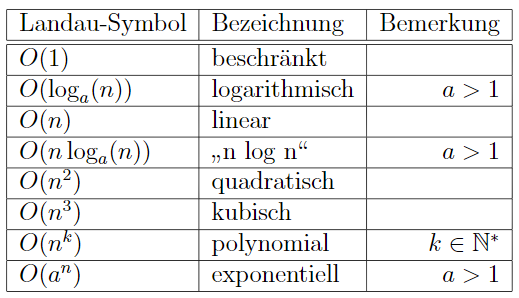
\includegraphics[width=7cm]{landau.PNG} \\
        \bottomrule
        
    \end{longtable}

\pagebreak

\subsection{Reihen}

    \begin{longtable}{p{0.75cm} p{1cm} p{16cm}}
        \toprule

        D & 5.5.1 &     Es sei $(a_n)$ eine Folge in $\mathbb{K}$. Dann heißt \hfill \break
                        \centerline{$\sum^{\infty}_{n=0} a_n = a_o + a_1 + a_2 + ... $}
                        die \textbf{Reihe} über $(a_n)$. \hfill \break
                        Für jedes $k \in \mathbb{N}$ heißt dann $s_k = \sum^{k}_{n=0} a_n$ die $k$-te Teilsumme oder \textbf{Partialsumme} der Reihe. \hfill \break
                        Ist die Folge $(s_k)_{k \in \mathbb{N}}$ konvergent, so nennen wir die Reihe \textbf{konvergent} mit dem Reihenwert: \hfill \break
                        \centerline{$\sum^{\infty}_{n=0} a_n := lim_{k \rightarrow \infty} s_k = lim_{k \rightarrow \infty} \sum^{k}_{n=0} a_n$}.
                        Ist $(s_k)$ divergent, so nennen wir auch die Reihe divergent.  \\
        \midrule
        S   & 5.5.3 &   Seien $\sum^{\infty}_{n=0} a_n$ und $\sum^{\infty}_{n=0} b_n$ zwei konvergente Reihen in $\mathbb{K}$ und 
                        $\alpha, \beta \in \mathbb{K}$. Dann ist auch $\sum^{\infty}_{n=0} (\alpha a_n + \beta b_n)$ konvergent und es gilt \hfill \break
                        \centerline{$\sum^{\infty}_{n=0} (\alpha a_n + \beta b_n) = \alpha \sum^{\infty}_{n=0} a_n + \beta \sum^{\infty}_{n=0} b_n$}  \\
        \midrule
        S   & 5.5.4 &   Es gilt $\sum^{\infty}_{n=0} \frac{1}{n!} = e$. \\
        \midrule
        S   & 5.5.5 &   Ist $\sum^{\infty}_{n=0} a_n$ eine konvergente Reihe in $\mathbb{K}$, so ist $(a_n)$ eine \textbf{Nullfolge} in $\mathbb{K}$. \\
        \midrule
        B   & 5.5.5 &   Gilt nicht umgekehrt. Nullfolge ist eine Voraussetzung für eine konvergente Reihe, aber keine Garantie. \\
        \midrule
        S   & 5.5.6 &   Es sei $(a_n)$ eine Folge in $\mathbb{K}$ und $s_k := \sum^{k}_{n=0} a_n$, $k \in \mathbb{N}$ Dann gilt:
                        \begin{itemize}[topsep=-0.5cm]
                            \item[a)] \textbf{Monotonie Kriterium} \hfill \break
                                        Ist $a_n \geq 0$ für alle $n \in \mathbb{N}$ und $(s_k)_{k \in \mathbb{N}}$ nach oben beschränkt, so
                                        ist $\sum^{\infty}_{n=0} a_n$ konvergent.
                            \item[b)] \textbf{Cauchy-Kriterium} \hfill \break
                                        Die Reihe $\sum^{\infty}_{n=0} a_n$ ist genau dann konvergent, wenn für jedes $\epsilon > 0$ ein $n_o \in \mathbb{N}$
                                        existiert mit \hfill \break
                                        \centerline{$|\sum^{k}_{n=l+1} a_n| < \epsilon$ für alle $k, l \in \mathbb{N}$ mit $k > l \geq n_0$.}
                        \end{itemize} \vspace{-0cm} \\
        \midrule
        S   & 5.5.7 &   \textbf{Leibniz-Kriterium} \hfill \break
                        Es sei $(a_n)$ eine monoton fallende Folge in $\mathbb{R}$ mit $lim_{n \rightarrow \infty} a_n = 0$. Dann ist die 
                        Reihe $\sum^{\infty}_{n=0} (-1)^n a_n$ konvergent. \\
        \midrule
        BSP &      &    \textbf{Reihen:}
                        \begin{itemize}[topsep=-0.5cm]
                            \item $\sum^{\infty}_{n=0} q^n = \frac{1}{1-q}, |q| < 1$ \textit{(Geometrische Reihe)}
                            \item $\sum^{\infty}_{n=1} \frac{1}{n(n+1)} = 1$
                            \item $\sum^{\infty}_{n=1} \frac{1}{n} = divergent$ \textit{(Harmonische Reihe)}
                            \item $\sum^{\infty}_{n=0} \frac{1}{n!} = e$
                            \item $\sum^{\infty}_{n=0} (-1)^n \frac{1}{n+1} = ln(2)$ \textit{(alternierende harmonische Reihe)} (Leibniz-Kriterium)
                            \item $\sum^{\infty}_{n=1} \frac{1}{n^{\alpha}}:$ konvergent, wenn $\alpha > 1$, sonst divergent
                        \end{itemize} \vspace{-0cm} \\
        \bottomrule

    \end{longtable}

\pagebreak

\subsubsection{Absolute Konvergenz}

    \begin{longtable}{p{0.75cm} p{1cm} p{16cm}}
        \toprule

        D   & 5.5.9 &   Eine Reihe $\sum^{\infty}_{n=0} a_n$ in $\mathbb{K}$ heißt \textbf{absolut konvergent}, wenn die Reihe
                        $\sum^{\infty}_{n=0} |a_n|$ in $\mathbb{K}$ konvergiert. (Summanden werden schnell genug klein, vorzeichenunabhängig)\\
        \midrule
        S   & 5.5.10&   Jede absolut konvergente Reihe $\sum^{\infty}_{n=0} a_n$ in $\mathbb{K}$ ist auch konvergent in $\mathbb{K}$ und es
                        gilt die verallgemeinerte Dreiecksungleichung \hfill \break
                        \centerline{$|\sum^{\infty}_{n=0}a_n| \leq \sum^{\infty}_{n=0} |a_n|$} \\
        \midrule
        B   & 5.5.10&   Gilt nicht umgekehrt (alternierende harmonische Reihe)  \\
        \midrule
        B   & 5.5.10&   Absolute Konvergenz: Reihenwert ist unabhängig von der Summationsreihenfolge \\
        \midrule
        S   & 5.5.12&   Es seien $(a_n)$ und $(b_n)$ reelle Folgen und $n_o \in \mathbb{N}$.
                        \begin{itemize}[topsep=-0.5cm]
                            \item \textbf{Majorantenkriterium} \hfill \break 
                                    Ist $|a_n| \leq b_n$ für alle $n \geq n_o$ und konvergiert die Reihe $\sum^{\infty}_{n=0}b_n$, so ist
                                    $\sum^{\infty}_{n=0} a_n$ absolut konvergent.
                            \item \textbf{Minorantenkriterium} \hfill \break
                                    Ist $a_n \geq b_n \geq 0$ für alle $n \geq n_0$ und divergiert die Reihe $\sum^{\infty}_{n=0}b_n$, so 
                                    divergiert auch die Reihe $\sum^{\infty}_{n=0}a_n$. 
                        \end{itemize} \vspace{-0cm} \\
        \midrule
        B   & 5.5.12&   Die Vergleichsfolge heißt jeweils konverente Majorante bzw. divergente Minorante. \\
        \midrule
        S   & 5.5.16&   Es sei $\sum^{\infty}_{n=0}a_n$ eine Reihe in $\mathbb{K}$.
                        \begin{itemize}[topsep=-0.5cm]
                            \item[a)] \textbf{Wurzelkriterium} \hfill \break
                                    Existiert der Grenzwert $lim_{n \rightarrow \infty} \sqrt[n]{|a_n|}$, so ist die Reihe
                                    \begin{itemize}[topsep=-0.5cm]
                                        \item absolut konvergent, wenn $lim_{n \rightarrow \infty} \sqrt[n]{|a_n|} < 1$ ist
                                        \item divergent, wenn $lim_{n \rightarrow \infty} \sqrt[n]{|a_n|} > 1$ ist
                                    \end{itemize}
                            \item[b)] \textbf{Quotientenkriterium} \hfill \break
                                    Ist $a_n \neq 0$ für alle $n \in \mathbb{N}$ und existiert der Grenzwert 
                                    $lim_{n \rightarrow \infty} |\frac{a_{n+1}}{a_n}|$, so ist die Reihe
                                    \begin{itemize}[topsep=-0.5cm]
                                        \item absolut konvergent, wenn $lim_{n \rightarrow \infty} |\frac{a_{n+1}}{a_n}| < 1$ ist
                                        \item divergent, wenn $lim_{n \rightarrow \infty} |\frac{a_{n+1}}{a_n}| > 1$ ist
                                    \end{itemize}
                        \end{itemize} \vspace{-0cm} \\
        \midrule
        B   & 5.5.16&   Liefert Wurzel-/Quotientenkriterium genau Eins, kann man daraus keine Aussage ableiten \\
        \bottomrule

    \end{longtable}

\subsubsection{Das Cauchy-Produkt}

    \begin{longtable}{p{0.75cm} p{1cm} p{16cm}}
        \toprule
         S   & 5.5.19&   Es seien $\sum^{\infty}_{n=0} a_n$ und $\sum^{\infty}_{n=0} b_n$ zwei \textbf{absolut konvergente Folgen} in $\mathbb{K}$.
                Dann konvergiert auch die Reihe $\sum^{\infty}_{n=0} \sum^{n}_{k=0} a_k b_{n-k}$ \textbf{absolut} und es gilt für
                die Reihenwerte: \hfill \break
                \centerline{$\sum\limits^{\infty}_{n=0} \sum\limits^{n}_{k=0} a_k b_{n-k} = (\sum\limits^{\infty}_{n=0} a_n) (\sum\limits^{\infty}_{n=0} b_n)$} 
                Die Reihe $\sum\limits^{\infty}_{n=0} \sum\limits^{n}_{k=0} a_k b_{n-k}$ heißt \textbf{Cauchy-Produkt} der beiden Reihen. \\
        \midrule
        S   & 5.5.20&   Für alle $z,w \in \mathbb{C}$ gilt $E(z+w) = E(z)E(w)$. \\
        \midrule
        D   & 5.5.21&   Für alle $z \in \mathbb{C}$ ist $e^z:= E(z) = \sum\limits^{\infty}_{n=0} \frac{z^n}{n!}$. \\

        \bottomrule

    \end{longtable}

\pagebreak

\subsection{Konvergenz in normierten Räumen}

    \begin{longtable}{p{0.75cm} p{1cm} p{16cm}}
        \toprule

        D   & 5.6.1 &   \begin{minipage}{\linewidth}
                            \begin{itemize}
                                \item[a)] Eine Folge $(a_n)_{n \in \mathbb{N}}$ in $V$ heißt \textbf{konvergent} gegen ein $a \in V$, wenn
                                            für jedes $\epsilon > 0$ ein $n_0 \in \mathbb{N}$ existiert, so dass \hfill \break
                                            \centerline{$||a_n - a||_V < \epsilon$ für alle $n \geq n_0$}
                                            Die Folge heißt \textbf{divergent,} wenn sie nicht konvergent ist.
                                \item[b)] Eine Folge heißt \textbf{Cauchy-Folge}, wenn es für jedes $\epsilon > 0$ ein $n_0 \in \mathbb{N}$ gibt
                                            mit \hfill \break
                                            \centerline{$||a_n - a_m||_V < \epsilon$ für alle $n,m \geq n_0$}
                                \item[c)] Eine Reihe $\sum^{\infty}_{n=0} a_n$ in $V$ heißt \textbf{konvergent} mit Reihenwert $s \in V$, wenn die
                                            Folge der Partialsummen $s_k := \sum^{k}_{n=0} a_n$, $k \in \mathbb{N}$, in $V$ gegen $s$ konvergiert. \hfill \break
                                            Konvergiert die Reihe $\sum^{\infty}_{n=0} ||a_n||_V$ in $\mathbb{R}$ so heißt die Reihe
                                            $\sum^{\infty}_{n=0}a_n$ \textbf{absolut konvergent}. \hfill \break
                                            Ist die Reihe nicht konvergent, so nennt man sie \textbf{divergent}.
                            \end{itemize}
                        \end{minipage} \\
        \midrule
        B   & 5.6.1 &   Genau dasselbe wie vorher, wir ersetzen nur den Betrag durch die jeweilige Norm \\
        \midrule
        B   & 5.6.1 &   \textbf{Cauchy-Folge}: Abstand von je zwei Folgegliedern \\
        \midrule
        B   &       &   \textbf{2-Norm}: $||x||_2 = \sqrt{x_1^2 + x_2^2}$ \\
        \midrule
        D   & 5.6.2 &   Eine Menge $M \subseteq V$ hei\ss t beschränkt, falls es ein $ \geq 0$ gibt, so dass $||x||_V \leq C$ für alle 
                        $x \in \mathbb{M}$ gilt. \\
        \midrule
        BSP & 5.6.3 &   $V = \mathbb{R}^3$, 1-Norm: $||x||_1 = \sum^3_{j=1} |x_i|$, $a_n := (1, \frac{1}{n}, \frac{n-1}{n})^T$, $n \in \mathbb{N^*}$ \hfill \break
                    Hier gilt $lim_{n \rightarrow \infty} a_n = (1,0,1)^T$. Zeige: Abstand von $a_n$ zu Grenzwert beliebig klein: \hfill \break
                    $||a_n - (1,0,1)^T|| = |0| + |\frac{1}{n}| + |\frac{n-1}{n}-1| = \frac{2}{n}$ (Abstand geht gegen 0) \hfill \break
                    Sei $\epsilon > 0$. Dann existiert $n_0 \in \mathbb{N}$ mit $n_0 > \frac{2}{\epsilon}$. Für alle $n \geq n_0$ gilt: \hfill \break
                    $||a_n - (1,0,1)^T||_1 = \frac{2}{n} \leq \frac{2}{n_0} \leq \frac{2\epsilon}{2} = \epsilon$ \\
        \midrule
        S   & 5.6.5 &   Es sei $(a_n)_{n \in \mathbb{N}} = ((a_{n,1}, a_{n,2}, \dots, a_{n,d})^T)_{n \in \mathbb{N}}$ eine Folge in $\mathbb{R}^d$
                    mit der 2-Norm. Dann ist $(a_n)$ in $\mathbb{R}^d$ genau dann \textbf{konvergent}, wenn für jedes $j \in \{1,2,\dots,d\}$ die
                    Koordinatenfolge $(a_{n,j})_{n \in \mathbb{N}}$ in $\mathbb{R}$ \textbf{konvergent} ist. In diesem Fall ist \hfill \break
                    \centerline{$lim_{n \rightarrow \infty}\begin{pmatrix}a_{n,1}\\a_{n,2}\\\dots \\ a_{n,d}\end{pmatrix} =
                        \begin{pmatrix} lim_{n \rightarrow \infty} a_{n,1} \\ lim_{n \rightarrow \infty} a_{n,2} \\ \dots \\
                        lim_{n \rightarrow \infty} a_{n,d} \end{pmatrix}$}.
                    Falls eine Komponente im Vektor divergiert, divergiert die ganze Folge. \\
        \midrule
        B   & 5.6.5 &   Der Satz gilt im endlichen Raum für alle Normen. \hfill \break
                    Wenn eine Folge bezüglich einer Norm konvergiert, dann auch bzgl jeder anderen. \hfill \break 
                    Grenzwerte bleiben gleich. \\
        \midrule
        D   & 5.6.8 &   \begin{minipage}{\linewidth}
                            \begin{itemize}
                                \item[a)] Es seien $x_0 \in \mathbb{V}$ und $r \in (0, \infty)$. Dann heißt die Menge \hfill \break
                                            $B_r(x_0) := \{x \in V: ||x-x_o||_V < r\} $ \textbf{(offene) Kugel} um $x_0$ (Mittelpunkt) mit Radius $r$.
                                \item[b)] Eine Menge $M \subseteq V$ heißt \textbf{offen}, falls es für jeden Punkt $x_0 \in M$ einen Radius
                                            $r > 0$ gibt, so dass $B_r(x_0) \subseteq M$ gilt.
                                \item[c)] Eine Menge $M \subseteq V$ heißt \textbf{abgeschlossen}, wenn die Menge $M^c = V \ M$ offen ist.
                                \item[d)] Es sei $M \subseteq V$. Ein Punkt $x_0 \in M$ heißt \textbf{innerer Punkt} von $M$, falls es ein
                                            $r > 0$ gibt, so dass $B_r(x_0) \subseteq M$ ist. \hfill \break 
                                            Man nennt $M^o := \{x \in M: x$ innerer Punkt von $M$\} das \textbf{Innere von $M$}.    
                            
                            \end{itemize}
                        \end{minipage} \\
        \midrule
        B   & 5.6.8 &   Menge \textbf{abgeschlossen}: Rand gehört zur Menge \hfill \break
                    Menge \textbf{offen}: Rand gehört nicht zur Menge \hfill \break
                    Die meisten Menge sind weder offen noch abgeschlossen, keine Umkehrschlüsse! \\
        \midrule
        S   & 5.6.11 &  Eine Teilmenge $M$ von $V$ ist genau dann \textbf{abgeschlossen}, wenn für jede Folge in $M$, die in $V$ konvergiert,
                    der Grenzwert ein Element aus $M$ ist. \\
        \midrule
        D   & 5.6.13&   Ist $V$ ein endlichdimensionaler normierter $\mathbb{R}$-Vektorraum, so hei\ss t eine Teilmenge $M \subseteq V$
                        \textbf{kompakt}, wenn sie abgeschlossen und beschränkt ist. \\
        \midrule
        D   & 5.6.15&   Es sei $(a_n)$ eine Folge in $(V, ||\cdot||_V)$.
                        \begin{itemize}[topsep=-0.5cm]
                            \item[a)] Ein $a \in V$ hei\ss t \textbf{Häufungswert} von $(a_n)$m falls für jedes $\epsilon > 0$ die Menge \hfill \break
                                        \centerline{\{$n \in \mathbb{N} : ||a_n - a||_V < \epsilon\} = \{n \in \mathbb{N}: a_n \in B_{\epsilon}(a)\}$}
                                        unendlich viele Elemente hat.
                            \item[b)] Ist $\{n_1,n_2,n_3,\dots\}$ eine unendliche Teilmenge von $\mathbb{N}$ mit $n_1 < n_2 < n_3 < \dots$, so
                                        hei\ss t $(a_{n_k})_{k \in \mathbb{N}}$ eine \textbf{Teilfolge} von $(a_n)$. 
                        \end{itemize} \vspace{-0cm} \\
        \midrule
        S   & 5.6.17&   \textbf{Satz von Bolzano-Weierstra\ss} \hfill \break
                    Sei $(V, ||\cdot||_V)$ ein endlichdimensionaler normierter Raum und $M \subseteq V$ kompakt. Dann besitzt jede Folge in $M$
                    eine \textbf{konvergente Teilfolge mit Grenzwert in $M$}. \\
        \midrule
        B   & 5.6.17&   Ist $(V,||\cdot||_V)$ ein endlichdimensionaler normierter Raum,so besitzt jede beschränkte Folge in 
                    $V$ mindestens einen Häufungswert. (Unendliche viele Punkte in einer beschränkten Menge müssen irgendwo klumpen) \\
        \midrule
        D   & 5.6.19&   Ein normierter $\mathbb{R}$-Vektorraum $(V, ||\cdot||_V)$ heißt \textbf{vollständig}, wenn jede Cauchy-Folge in $V$ konvergiert.
                        Ein vollständiger normierter $\mathbb{R}$-Vektorraum wird auch \textbf{Banachraum} genannt. \hfill \break
                        Wird die Norm $||\cdot||_V$ außerdem durch eine Skalarprodukt auf $V$ induziert, so nennt man $V$ \textbf{Hilbertraum}. \\
        \midrule
        B   & 5.6.19&   Standardvektorraum $\mathbb{R}^d$ ist für jedes $d \in \mathbb{N^*}$ mit jeder Norm ein \textbf{Banachraum}. \hfill \break
                    Wählt man au\ss erdem die durch das Skalarprodukt induzierte 2-Norm, so ist $(\mathbb{R}^d, ||\cdot||_2)$ ein \textbf{Hilbertraum}. \\

        \bottomrule
        B   &       &   Normierter Raum: $V$ = normierter Vektorraum mit Norm $||\cdot||_V$ (ermöglicht Abstandsmessung) \hfill \break
                    Hier als Vorstellung $\mathbb{R}^3$ mit Standard(2)-Norm (normaler Abstand im Raum) \\
        \midrule
        S   & 5.6.22&   \textbf{Banach'scher Fixpunktsatz} \hfill \break
                    Es sei $(V, ||\cdot||_V)$ ein Banachraum $M \subseteq V$ abgeschlossen und $f: M \rightarrow M$ eine Funktion.
                    Weiter existiere ein $q \in (0,1)$, so dass \hfill \break
                    \centerline{$||f(x) - f(y)||_V \leq q ||x-y||_V$, für alle $x,y \in M$}
                    gilt. Dann gelten die folgenden Aussagen:
                    \begin{itemize}[topsep=-0.5cm]
                        \item[a)] Es gibt genau ein $v \in M$ mit $f(v) = v$. (d.h. $f$ hat genau einen Fixpunkt in M)
                        \item[b)] Für jedes $x_0 \in M$ konvergiert die Folge $(x_n)$ mit $x_{n+1} = f(x_n)$, $n \in \mathbb{N}$, gegen $v$
                                    und es gelten die folgenden Fehlerabschätzungen für hedes $n \in \mathbb{N^*}$:
                                    \begin{itemize}[topsep=-0.5cm]
                                        \item[] $||x_n-v||_V \leq \frac{q^n}{1-q}||x_1-x_0||_V$ (A-priori-Abschätzung)
                                        \item[] $||x_n-v||_V \leq \frac{q}{1-q}||x_n-x_{n-1}||_V$ (A-posterior-Abschätzung)
                                    \end{itemize}
                    \end{itemize} \vspace{-0cm} \\

        \bottomrule

    \end{longtable}

\pagebreak

\subsection{Stetigkeit reeller Funktionen}
\subsubsection{Der Grenzwertbegriff für Funktionen}

    \begin{longtable}{p{0.75cm} p{1cm} p{16cm}}
        \toprule

        D   & 5.7.1 &   Es sei $D \subseteq \mathbb{R}$ eine Menge, $f: D \rightarrow \mathbb{R}$ eine Funktion und $x_0 \in \mathbb{R}$
                        \begin{itemize}[topsep=-0.5cm]
                            \item[a)] Wir nennen $x_0$ einen \textbf{Häufungspunkt} von $D$, falls es eine Folge $(a_n)$ in $D$ mit
                                        $a_n \neq x_0$ für alle $n \in \mathbb{N}$ gibt, die gegen $x_0$ konvergiert.
                            \item[b)] Ist $x_0$ ein Häufungspunkt von $D$, so sagen wir, dass $f$ für $x$ gegen $x_0$ den Grenzwert 
                                        $y$ hat, wenn für jede Folge $(a_n)$ in $D$, die gegen $x_0$ konvergiert und für die
                                        $a_n \neq x_0$ für alle $n \in \mathbb{N}$ gilt, die Folge $(f(a_n))$ gegen $y$ konvergiert.
                                        \hfill \break Wir schreiben dafür: $lim_{x \rightarrow x_0} f(x) = y$.
                            \item[c)] Ist $x_0$ ein Häufungspunkt von $D_+ := \{ x \in D : x > x_0\}$, so hat $f$ für $x$ gegen $x_0$
                                        den \textbf{rechtsseitigen Grenzwert} $y$, wenn für jede Folge $(a_n)$ in $D_+$, die gegen
                                        $x_0$ konvergiert, die Folge $(f(a_n))$ gegen $y$ konvergiert.
                                        \hfill \break Wir schreiben dafür: $lim_{x \rightarrow x_{0+}} f(x) = y$.
                            \item[d)] Ist $x_0$ ein Häufungspunkt von $D_- := \{ x \in D : x < x_0\}$, so hat $f$ für $x$ gegen $x_0$
                                        den \textbf{linksseitigen Grenzwert} $y$, wenn für jede Folge $(a_n)$ in $D_-$, die gegen
                                        $x_0$ konvergiert, die Folge $(f(a_n))$ gegen $y$ konvergiert.
                                        \hfill \break Wir schreiben dafür: $lim_{x \rightarrow x_{0-}} f(x) = y$.
                        \end{itemize} \vspace{-0cm} \\
        \midrule
        B   & 5.7.1 &   $x_0$ HP von $D$ bedeutet, dass $x_0$ aus $D$ $\textbackslash$ \{$x_o$\} annäherbar \hfill \break
                        Bsp.: HP von $(0,1]$: $[0,1]$ \\
        \midrule
        S   & 5.7.4 &   Es sei $D \subseteq \mathbb{R}$, $f: D \rightarrow \mathbb{R}$ eine Funktion und $x_0 \in \mathbb{R}$. 
                        Existieren $lim_{x \rightarrow x_{0-}}f(x)$ und $lim_{x \rightarrow x_{0+}}f(x)$ und sind die beiden Werte gleich
                        so existiert auch $lim_{x \rightarrow x_0} f(x)$ und es gilt \hfill \break
                        \centerline{$lim_{x \rightarrow x_0} f(x) = lim_{x \rightarrow x_{0-}} = lim_{x \rightarrow x_{0+}}$}.  \\
        \midrule
        B   & 5.7.4 &   Es gilt nicht $lim_{x \rightarrow x_0}f(x) = f(x_0)$. \\
        \midrule
        S   & 5.7.6 &   Es sei $D \subseteq \mathbb{R}$ und $x_0$ ein Häufungspunkt von $D$. Desweiteren seien drei Funktionen $f,g,h:
                        D \rightarrow \mathbb{R}$ gegeben, so dass die Grenzwerte $lim_{x \rightarrow x_0} f(x)$ und
                        $lim_{x \rightarrow x_0} g(x)$ existieren. Dann gilt:
                        \begin{itemize}[topsep=-0.5cm]
                            \item[a)] Die Grenzwerte für $x$ gegen $x_0$ von $f+g$, $fg$ und $|f|$ existieren und es gilt:
                                \begin{itemize}[topsep=-0.5cm]
                                    \item $lim_{x \rightarrow x_0} (f(x) + g(x)) = lim_{x \rightarrow x_0} f(x) + lim_{x \rightarrow x_0} g(x)$
                                    \item $lim_{x \rightarrow x_0} (f(x) \cdot g(x)) = lim_{x \rightarrow x_0} f(x) \cdot lim_{x \rightarrow x_0} g(x)$
                                    \item $lim_{x \rightarrow x_0} |f(x)| = |lim_{x \rightarrow x_0} f(x)|$
                                \end{itemize}
                            \item[b)] Gilt $f(x) \leq g(x)$ für alle $x \in D \textbackslash \{x_0\}$, so ist $lim_{x \rightarrow x_0} f(x)
                                        \leq lim_{x \rightarrow x_0}g(x)$
                            \item[c)] Ist $lim_{x \rightarrow x_0} f(x) = lim_{x \rightarrow x_0} g(x)$ und es gilt 
                                        $f(x) \leq h(x) \leq g(x)$ für alle $x \in D \textbackslash \{x_0\}$, so gilt auch
                                        $lim_{x \rightarrow x_0} h(x) = lim_{x \rightarrow x_0}f(x) = lim_{x \rightarrow x_0}g(x)$.
                                        (Sandwich-Theorem)
                            \item[d)] Ist $y := lim_{x \rightarrow x_0} g(x) \neq 0$, so existiert $\delta > 0$, so dass
                                        $|g(x)| \geq \frac{|y|}{2}$ für alle $x \in (D \cap (x_0 - \delta, x_0 + \delta)) \textbackslash \{x_0\}$
                                        ist. Wir können also die Funktion $\frac{f}{g}: (D \cap (x_0 - \delta, x_0 + \delta)) \textbackslash \{x_0\}
                                        \rightarrow \mathbb{R}$ mit $\frac{f}{g}(x) := \frac{f(x)}{g(x)}$ definieren. Für diese existiert dann
                                        der Limes für $x$ gegen $x_0$ mit $lim_{x \rightarrow x_0} \frac{f(x)}{g(x)} = 
                                        \frac{lim_{x \rightarrow x_0}f(x)}{lim_{x \rightarrow x_0}g(x)}$.
                        \end{itemize} \vspace{-0cm} \\
        \midrule
        D   & 5.7.7 &   \textbf{Divergenz}
                        \begin{itemize}[topsep=-0.5cm]
                            \item[a)] Es seien $D \subseteq \mathbb{R}$, $f: D \rightarrow \mathbb{R}$ eine Funktion und $x_0$ ein
                                        Häufungspunkt von $D$. Wir schreiben $lim_{x \rightarrow x_0}f(x) = \infty (-\infty)$, wenn
                                        für jedes Folge $(a_n)$ in $D$, die gegen $x_0$ konvergiert und für die $a_n \neq x_0$ für 
                                        alle $n \in \mathbb{N}$ gilt, die Folge $(f(a_n))$ bestimmt gegen $\infty (-\infty)$ divergiert.
                            \item[b)] Es sei $D \subset \mathbb{R}$ \textbf{nicht} nach oben (unten) \textbf{beschränkt}, 
                                        $f : D \rightarrow \mathbb{R}$ eine Funktion und $y \in \mathbb{R} \cup \{\infty,-\infty\}$. 
                                        Wir sagen $lim_{x \rightarrow \infty} f(x) = y$ (bzw. $lim_{x \rightarrow -\infty} f(x) = y$),
                                        wenn für jede Folge $(a_n)$ in $D$, die bestimmt gegen $\infty (-\infty)$ divergiert,
                                        $lim_{n \rightarrow \infty} f(a_n) = y$ gilt.
                        \end{itemize} \vspace{-0cm} \\
        \midrule
        BSP & 5.7.8 &   $lim_{x \rightarrow \infty} \frac{1}{x} = 0$ \hfill \break
                        $lim_{x \rightarrow 0+} \frac{1}{x} = \infty$ \hfill \break
                        $lim_{x \rightarrow 0-} \frac{1}{x} = -\infty$ \hfill \break
                        $lim_{x \rightarrow \infty} x = \infty$ \\
        \midrule
        BSP & 5.7.8 &   Exponentialfunktion: $E(x) = e^x = \sum^{\infty}_{n=0} \frac{x^n}{n!}$ \hfill \break
        Grenzwerte: \hfill \break
        $lim_{x \rightarrow \infty} e^x = \infty$ \hfill \break
        $lim_{x \rightarrow -\infty} e^x = 0$ \\

        \bottomrule

    \end{longtable}

\subsubsection{Stetigkeit}

\begin{longtable}{p{0.75cm} p{1cm} p{16cm}}
        \toprule

        D   & 5.7.9 &   Es sei $D \subseteq \mathbb{R}$ und $x_0 \in D$. Eine Funktion $f : D \rightarrow \mathbb{R}$ heißt
                        \textbf{stetig} in $x_0$, falls für jede Folge $(a_n)$ in $D$, die gegen $x_0$ konvergiert, auch die Folge $(f(a_n))$ 
                        konvergiert und $lim_{n \rightarrow \infty} f(a_n) = f(x_0)$ gilt. \hfill \break 
                        Weiter heißt $f$ stetig auf $D$, wenn $f$ in jedem Punkt $x_0 \in D$ stetig ist. \hfill \break
                        Schließlich setzen wir noch $C(D) := \{f:D \rightarrow \mathbb{R}: f$ stetig auf $D\}$. 
                        (Menge aller stetigen Funktionen auf D) \\
        \midrule
        B   & 5.7.9 &   Stetigkeit: Kleines Wackeln an Parametern $\rightarrow$ auch nur kleines Wackeln am Funktionswert \\
        \midrule
        S   & 5.7.12&   Es sei $D \subseteq \mathbb{R}$ und $f : D \rightarrow \mathbb{R}$ eine Funktion. Ist $x_0 \in D$ ein Häufungspunkt
                        von D,so ist $f$ in $x_0$ genau dann \textbf{stetig}, wenn $lim_{x \rightarrow x_0} f(x) = f(x_0)$ gilt. \\
        \midrule
        B   & 5.7.12&   Stetigkeit: Grenzübergang austauschbar mit Funktionsauswertung \\
        \midrule
        S   & 5.7.15&   Es sei $D \subseteq \mathbb{R}$ und $f,g : D \rightarrow \mathbb{R}$ seien stetig in $x_0 \in D$. Dann sind die
                        Funktionen $f+g$, $fg$ und $|f|$ stetig in $x_0$. \hfill \break
                        Ist $x_0 \in D^* := \{ x \in D: g(x) \neq 0\}$, so ist die Funktion $\frac{f}{g}:D^* \rightarrow \mathbb{R}$ stetig in $x_0$.\\
        \midrule
        B   & 5.7.15&   Jede Polynomfunktion ist auf ganz $\mathbb{R}$ stetig. \\
        \midrule
        S   & 5.7.16&   Es seien $D,E \subseteq \mathbb{R}$ und $f: D \rightarrow E$, sowie $g: E \rightarrow \mathbb{R}$ Funktionen. Ist $f$ 
                        stetig in $x_0 \in D$ und $g$ stetig in $f(x_0)$, so ist $g \circ f: D \rightarrow \mathbb{R}$ stetig in $x_0$. \\ 
        \midrule
        D   & 5.7.18&   Es sei $D \subseteq \mathbb{R}$. Eine Funktion $f: D \rightarrow \mathbb{R}$ heißt
                        \begin{itemize}[topsep=-0.5cm]
                            \item[a)] \textbf{monoton wachsend}, falls für alle $x,y \in D$ gilt $x \leq y \Rightarrow f(x) \leq f(y)$
                            \item[b)] \textbf{monoton fallend}, falls für alle $x,y \in D$ gilt $x \leq y \Rightarrow f(x) \geq f(y)$
                            \item[c)] \textbf{streng monoton wachsend}, falls für alle $x,y \in D$ gilt $x < y \Rightarrow f(x) < f(y)$
                            \item[d)] \textbf{streng monoton fallend}, falls für alle $x,y \in D$ gilt $x < y \Rightarrow f(x) > f(y)$
                            \item[e)] \textbf{(streng) monoton}, wenn sie (streng) monoton wachsend oder (streng) monoton fallend ist 
                        \end{itemize} \vspace{-0cm} \\
        \midrule
        B   & 5.7.19&   Exponentialfunktion ist streng monoton wachsend. \\
        \midrule
        S   & 5.7.20&   Es sei $D \subseteq \mathbb{R}$ und $x_0 \in D$. Eine Funktion $f: D \rightarrow \mathbb{R}$ ist in $x_0$ genau dann
                        \textbf{stetig}, wenn es für jedes $\epsilon > 0$ ein $\delta > 0$ gibt, so dass \hfill \break
                        \centerline{$|f(x) - f(y)| < \epsilon$ für alle $x \in D$ mit $|x-x_0|<\delta$ gilt.} \\
        \midrule
        D   & 5.7.22&   Es sei $D \subseteq \mathbb{R}$. Eine Funktion $f : D \rightarrow \mathbb{R}$ heißt \textbf{Lipschitz-stetig}, falls
                        es ein $L > 0$ gibt mit $|f(x) - f(y)| \leq L|x-y|$ für alle $x,y \in D$. \\
        \midrule
        S   & 5.7.23&   Ist $D \subseteq \mathbb{R}$ und $f:D \rightarrow \mathbb{R}$ \textbf{Lipschitz-stetig} so ist $f$ \textbf{stetig} auf $D$.
                        Die Umkehrung dieser Aussage ist falsch. (Lipschitz-Stetigkeit ist damit ein strengerer Begriff als Stetigkeit) \\
        \midrule
        B   & 5.7.23&   Lipschitz-Stetigkeit bedeutet anschaulich, dass die Steigung des Graphen beschränkt bleibt. \\
        \bottomrule

    \end{longtable}

\pagebreak

\subsubsection{Eigenschaften stetiger Funktionen}

    \begin{longtable}{p{0.75cm} p{1cm} p{16cm}}
        \toprule
        S   & 5.7.25&   \textbf{Zwischenwertsatz} \hfill \break
                        Es seien $a,b \in \mathbb{R}$ mit $a < b$ gegeben und $f \in C([a,b])$. Ist $y_0$ eine reelle Zahl zwischen $f(a)$ und $f(b)$,
                        so gibt es ein $x_0 \in [a,b]$ mit $f(x_0) = y_0$. \hfill \break
                        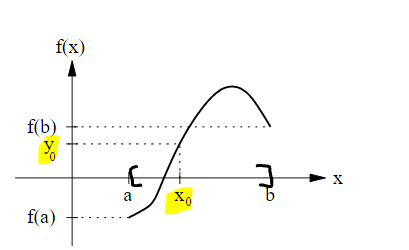
\includegraphics[width=3.5cm]{zws.png} \\
        \midrule
        S   & 5.7.26&   \textbf{Nullstellensatz von Bolzano} \hfill \break
                        Es seien $a,b \in \mathbb{R}$ mit $a < b$ gegeben und $f \in C([a,b])$ erfülle $f(a)f(b) < 0$ (Existenz einer Nullstelle /
                        Einer der beiden Werte 0).
                        Dann gibt es ein $x_0 \in (a,b)$ mit $f(x_0) = 0$. \\
        \midrule
        D   & 5.7.27&   Es sei $D \subseteq \mathbb{R}$. Eine Funktion $f: D \rightarrow \mathbb{R}$ hei\ss t beschränkt, falls die Menge
                        $f(D)$ (Bild der Funktion) beschränkt ist, d.h. falls ein $C \geq 0$ existiert, so dass $|f(x)| \leq C$ für alle $x \in D$ gilt. \\
        \midrule
        S   & 5.7.28&   Es sei $K \subseteq \mathbb{R}$ \textbf{kompakt} und nicht-leer, sowie $f \in C(K)$. Dann gibt es $x_*, x^* \in K$, so dass
                        $f(x_*) \leq f(x) \leq f(x^*)$ für alle $x \in K$ gilt. Insbesondere ist $f$ \textbf{beschränkt}. (Jede stetige Funktion auf 
                        kompakter Menge ist beschränkt)\\
        \bottomrule

    \end{longtable}


\subsection{Stetigkeit von Funktionen mehrerer Variablen}

    \begin{longtable}{p{0.75cm} p{1cm} p{16cm}}
        \toprule

        D   & 5.8.1 &   Es seien $V$ und $W$ normierte $\mathbb{R}$-Vektorräume, $D \subseteq V$ und $f: D \rightarrow W$ eine Funktion.
                \begin{itemize}[topsep=-0.5cm]
                    \item[a)] Wir nennen $x_0 \in D$ \textbf{Häufungspunkt} von $D$, falls es eine Folge $(a_n)$ in $D$ mit 
                                $a_n \neq x_0$ für alle $n \in \mathbb{N}$ gibt, die gegen $x_0$ konvergiert.
                    \item[b)] Sei $x_0$ ein Häufungspunkt von $D$. Dann ist $lim_{x \rightarrow x_0} f(x) = y$, falls für jede 
                                Folge $(a_n)$ in $D$, die gegen $x_0$ konvergiert und $a_n \neq x_0$ für alle $n \in \mathbb{N}$
                                erfüllt, die Folge $(f(a_n))$ gegen $y$ konvergiert.
                \end{itemize} \vspace{-0cm} \\
        \midrule
        B   & 5.8.2 &   Hier keine links- und rechtsseitiger Grenzwerte, da es Unmengen an Richtungen gibt \\
        \midrule
        D   & 5.3.3 &   Es seien $V,W$ zwei normierte $\mathbb{R}$-Vektorräumen, $D \subseteq V$ und $x_0 \in D$. Eine Funktion $f: D\rightarrow W$
                        heißt \textbf{stetig} in $x_0$, wenn für jede Folge $(a_n)$ in $D$, die gegen $x_0$ konvergiert, auch die Folge
                        $(f(a_n))$ konvergiert und $lim_{n \rightarrow \infty} f(a_n) = f(x_0)$ gilt. \hfill \break
                        Weiter heißt \textbf{f stetig auf D}, wenn $f$ in jedem Punkt $x_0 \in D$ stetig ist. \hfill \break
                        Au\ss erdem setzen wir wieder $C(D;W) := \{f: D\rightarrow W: f$ stetig auf $D$\}. \\
        \midrule
        S   & 5.8.4 &   Es sei $D \subseteq \mathbb{R}^d$ und $x_0 \in D$. Dann ist $f: D \rightarrow \mathbb{R}^p$ genau dann in $x_0$
                        \textbf{stetig}, wenn alle Koordinatenfunktionen $f_1, f_2, \dots, f_p : D \rightarrow \mathbb{R}$ in $x_0$ stetig sind. \\
        \midrule
        S   & 5.8.5 &   Es seien $D \subseteq \mathbb{R}^d$, $x_0 \in D$ und $f,g : D \rightarrow \mathbb{R}$ stetig in $x_0$, sowie
                        $h : f(D) \rightarrow \mathbb{R}$ stetig in $f(x_0)$. Dann sind auch $f+g$, $fg$ und $h \circ f$ als Funktionen
                        von $D$ nach $\mathbb{R}$ stetig in $x_0$. \hfill \break
                        Ist au\ss erdem $x_0 \in D^* := \{x \in D: g(x) \neq 0\}$, so ist auch $\frac{f}{g}:D^* \rightarrow \mathbb{R}$ stetig in $x_0$. \\
        \midrule
        S   & 5.8.8 &   Es sei $K \subseteq \mathbb{R}^d$ \textbf{kompakt} und nicht-leer, sowie $f \in C(K)$. Dann gibt es $x_*, x^* \in K$, so dass \hfill \break
                        \centerline{$f(x_*) \leq f(x) \leq f(x^*)$ für alle $x \in K$}
                        gilt. Insbesondere ist $f$ \textbf{beschränkt}. \\
        \midrule
        S   & 5.8.10&   Es sei $||\cdot||$ irgendeine Norm auf $\mathbb{R}^d$ und $||\cdot||_2$ die 2-Norm auf $\mathbb{R}^d$. Dann gibt es zwei Konstanten
                        $c$ und $C$ mit $0 < c \leq C$, so dass $c||x||_2  \leq ||x|| \leq C ||x||_2$ für alle $x \in \mathbb{R}^d$ gilt. \\
        \midrule
        S   & 5.8.11&   \begin{minipage}{\linewidth}
                            \begin{itemize}
                                \item[a)] Sind $||\cdot||$ und $|||\cdot|||$ zwei Normen auf $\mathbb{R}^d$, so gibt es Konstanten $0 < c \leq C$, so dass
                                            $c||x|| \leq |||x||| \leq C||x||$ für alle $x \in \mathbb{R}^d$ gilt.
                                \item[b)] Ist eine Folge $(a_n)$ in $\mathbb{R}^d$ bezüglich einer Norm konvergent, so konvergiert sie auch bezüglich  
                                            jeder anderen Norm und der Grenzwert ist derselbe. 
                            \end{itemize}
                        \end{minipage} \\
        \midrule
        B   & 5.8.11&   Gilt $c||x|| \leq |||x||| \leq C||x||$ so hei\ss en die Normen $||\cdot||,|||\cdot|||$ äquivalent. \hfill \break
                        Je zwei Normen im $\mathbb{R}^d$ sind äquivalent. \\
        \bottomrule

    \end{longtable}

\pagebreak

\subsection{Potenzreihen}

    \begin{longtable}{p{0.75cm} p{1cm} p{16cm}}
        \toprule

        D   & 5.9.1 &   Es sei $(a_n)$ eine Folge $\mathbb{K}$. Eine Reihe der Form $\sum^{\infty}_{n=0} a_n x^n = a_0 + a_1x+a_2x^2+ \dots$ 
                        heißt \textbf{Potenzreihe}. \\
        \midrule
        B   &       &   Offensichtlich konvergieren alle Potenzreihen für $x = 0$. \\
        \midrule
        BSP & 5.9.2 &   \textbf{Geometrische Reihe} \hfill \break 
                        Konvergiert für $|x| < 1$ mit $\sum^{\infty}_{n=0} x^n = \frac{1}{1-x}$. \\
        \midrule
        BSP & 5.9.2 &   \textbf{Exponentialfunktion} \hfill \break
                        $e^z = \sum^{\infty}_{n=0} \frac{z^n}{n!}$ konvergiert für alle $z \in \mathbb{C}$ \\ 
        \midrule
        S   & 5.9.3 &   \textbf{Satz von Hadamard} \hfill \break
                        Es sei $(a_n)$ eine Folge in $\mathbb{K}$, so dass der Grenzwert $\rho := lim_{n \rightarrow \infty} \sqrt[n]{|a_n|}$ existiert
                        oder die Folge $(\sqrt[n]{|a_n|})$ unbeschränkt ist. Dann gelten die folgenden Konvergenzaussagen für die Potenzreihe 
                        $\sum^{\infty}_{n=0} a_n x^n$:
                        \begin{itemize}[topsep=-0.5cm]
                            \item[a)] Ist die Folge $\sqrt[n]{|a_n|}$ unbeschränkt, so konvergiert die Potenzreihe nur für \textbf{$x = 0$}.
                            \item[b)] Ist $\rho = 0$, so konvergiert die Potenzreihe für alle $x \in \mathbb{K}$ absolut. 
                            \item[c)] Ist $\rho \in (0, \infty)$, so ist die Potenzreihe für alle $x \in \mathbb{K}$ mit $|x|< \frac{1}{\rho}$
                                        \textbf{absolut konvergent} und für alle $x \in \mathbb{K}$ mit $|x| > \frac{1}{\rho}$ \textbf{divergent}.
                        \end{itemize} \vspace{-0cm} \\
        \midrule
        B   & 5.9.3 &   Keine Aussage bei $|x|=\frac{1}{\rho}$ möglich. \\
        \midrule
        B   & 5.9.3 &   Konvergenzbereich entweder $\{0\}$ oder $\mathbb{K}$ oder Kreis in $\mathbb{C}$ bzw. Intervall in $\mathbb{R}$ \\
        \midrule
        D   & 5.9.4 &   Es sei $\sum^{\infty}_{n=0} a_nx^n$ eine Potenzreihe die die Voraussetzungen von 5.9.3 erfüllt und $\rho$ wie in diesem Satz 
                        definiert. Dann heißt die Zahl: \hfill \break
                        \centerline{$r:=    \begin{cases}
                                            0 & \text{falls in obigem Satz a) gilt} \\
                                            \infty & \text{falls in obigem Satz b) gilt} \\
                                            \frac{1}{\rho} & \text{falls in obigem Satz c) gilt}
                                            \end{cases}$ }
                        der \textbf{Konvergenzradius} der Reihe. \\
        \midrule
        BSP & 5.9.5 &   \begin{minipage}{\linewidth}
                            \begin{itemize}
                                \item[a)] $a_n = 1$, $\sum^{\infty}_{n=0} x^n$ \hfill \break
                                            Dann gilt: $\rho = lim_{n \rightarrow \infty} \sqrt[n]{|a_n|} = lim_{n \rightarrow \infty} 1 = 1$, also $r = \frac{1}{\rho} = 1$. \hfill \break
                                            Am Rand: Für $x=1$: $\sum^{\infty}_{n=0} 1^n$ divergent. (-1 auch divergent) \hfill \break
                                            Konvergenzbereich: $(-1,1)$
                                \item[b)] $a_n = \frac{1}{n}$, $\sum^{\infty}_{n=1} \frac{x^n}{n}$ \hfill \break
                                            Konvergenzradius 1, da: $lim_{n \rightarrow \infty} \sqrt[n]{\frac{1}{n}} = lim_{n \rightarrow \infty} \frac{1}{\sqrt[n]{n}}
                                            = \frac{1}{lim_{n \rightarrow \infty} \sqrt[n]{n}} = 1$. \hfill \break
                                            Am Rand: Für $x=1$: $\sum^{\infty}_{n=1} \frac{1}{n}$: divergent (harmonische Reihe) \hfill \break
                                            Für $x=-1$: $\sum^{\infty}_{n=1} \frac{(-1)^n}{n}$: konvergent (alternierende harmonische Reihe) \hfill \break
                                            Konvergenzbereich: $[-1,1)$
                            \end{itemize}
                        \end{minipage}\\
        \midrule
        D   & 5.9.6 &   Es sei $(a_n)$ eine Folge in $\mathbb{K}$, $n_0 \in \mathbb{N}$ und $x_o \in \mathbb{K}$. Dann nennt man eine Reihe der Form \hfill \break
                        \centerline{$\sum^{\infty}_{n=n_0}a_n(x-x_0)^n$}
                        \textbf{Potenzreihe}. Der Punkt $x_0$ wird \textbf{Entwicklungspunkt} der Potenzreihe genannt. \hfill \break
                        (Hier ist das Konvergenzgebiet nun um $x_0$ statt um 0 (allgemeiner)) \hfill \break
                        (Alle Sätze und Definitionen gelten hier genauso) \\
        \midrule
        B   & 5.9.6 &   Konvergenzradius nun entweder $0$, $\infty$ oder $r = (lim_{n \rightarrow \infty} \sqrt[n]{|a_n|})^{-1}$. \\
        \midrule
        BSP & 5.9.6 &   $a_n := \frac{(-4)^n}{n}$, $x_0 = 1$, $\sum^{\infty}_{n=1} \frac{(-4)^n}{n}(x-1)^n$ \hfill \break
                        Es gilt: $\rho = lim_{n \rightarrow \infty} \sqrt[n]{|a_n|} = lim_{n \rightarrow \infty} \sqrt[n]{|\frac{(-4)^n}{n}|} =
                        lim_{n \rightarrow \infty} \frac{4}{\sqrt[n]{n}} = \frac{4}{1} = 4$ \hfill \break 
                        Konvergenzradius: $r = \frac{1}{\rho} = \frac{1}{4}$ \hfill \break
                        Konvergenz in $(1- \frac{1}{4}, 1 + \frac{1}{4}) = (\frac{3}{4}, \frac{5}{4})$ \hfill \break
                        Randpunkte: \hfill \break
                        $x = \frac{5}{4}:$ $\sum^{\infty}_{n=1} \frac{(-4)^n}{n}(\frac{5}{4}-1)^n = \sum^{\infty}_{n=1} \frac{(-4)^n}{n} \cdot \frac{1}{4^n}
                        = \sum^{\infty}_{n=1} \frac{(-1)^n}{n}$ konvergent (alt. harmonische Reihe)
                        $x = \frac{3}{4}:$ $\sum^{\infty}_{n=1} \frac{(-4)^n}{n}(\frac{3}{4}-1)^n = \sum^{\infty}_{n=1} \frac{(-4)^n}{n} \cdot \frac{1}{(-4)^n}
                        = \sum^{\infty}_{n=1} \frac{1}{n}$ divergent (harmonische Reihe) \hfill \break
                        Konvergenzgebiet: $(\frac{3}{4}, \frac{5}{4}]$\\
        \midrule
        S   & 5.9.10&   \textbf{Quotientenkriterium} \hfill \break
                    Es sei $(a_n)$ eine Folge in $\mathbb{K}$ mit $a_n \neq 0$ für alle $n \in \mathbb{N}$, so dass $\sigma := lim_{n \rightarrow \infty}
                    |\frac{a_{n+1}}{a_n}|$ existiert. Dann gilt für den Konvergenzradius r von $\sum^{\infty}_{n=0} a_n x^n$: \hfill \break
                    \centerline{$r =    \begin{cases}
                                        \frac{1}{\sigma}, & \text{falls } \sigma \in (0,\infty) \\
                                        \infty, & \text{falls } \sigma = 0.
                                        \end{cases}$} \\
        \midrule
        BSP & 5.9.11&   \begin{minipage}\linewidth
                            \begin{itemize}
                                \item[a)] $a_n = \frac{n^n}{n!}$, $\sum^{\infty}_{n=0} \frac{n^n}{n!}x^n$ \hfill \break
                                            Quotientenkriterium:  \hfill \break
                                            $\sigma := lim_{n \rightarrow \infty} |\frac{a_{n+1}}{a_n}| = lim_{n \rightarrow \infty} 
                                            |\frac{(n+1)^{n+1}}{(n+1)!} \cdot \frac{n!}{n^n}| = lim_{n \rightarrow \infty} | \frac{(n+1) \cdot (n+1)^n}{(n+1) n}| =
                                            lim_{n \rightarrow \infty}(\frac{n+1}{n})^n = lim_{n \rightarrow \infty} (1 + \frac{1}{n})^n = e$  \hfill \break
                                            Konvergenzradius: $r = \frac{1}{\sigma} = \frac{1}{e}$ \hfill \break
                                \item[b)] $\sum^{\infty}_{n=0} \frac{1}{2^n} x^{3n}$ Achtung Falle! Wegen $3^n$ kein Hadamard und 5.9.10 anwendbar. \hfill \break
                                            Substitution $y = x^3$. $\rightarrow \sum^{\infty}_{n=0} \frac{1}{2^n} y^{n}$ \hfill \break
                                            Konvergenzradius: 2, da $lim_{n \rightarrow \infty} \sqrt[n]{|\frac{1}{2^n}|} = \frac{1}{2}$. \hfill \break
                                            Also Konvergenz für $y = x^3 \in (-2,2)$, Divergenz außerhalb $[-2,2]$ \hfill \break
                                            $\rightarrow$ Konvergenz für $x \in (-\sqrt[3]{2},\sqrt[3]{2})$, Divergenz außerhalb $[-\sqrt[3]{2},\sqrt[3]{2}]$ \hfill \break
                                            Konvergenzradius der ursprünglichen Reihe ist $\sqrt[3]{2}$. 
                            \end{itemize}
                        \end{minipage} \\
        \midrule
        S   & 5.9.13&   \textbf{Cauchy-Produkt von Potenzreihen} \hfill \break
                        Es seien $\sum^{\infty}_{n=0}a_n x^n$ und $\sum^{\infty}_{n=0} b_n x^n$ Potenzreihen in $\mathbb{K}$ mit Konvergenzradien $r_1, r_2 >0$.
                        Dann hat die Potenzreihe \hfill \break
                        \centerline{$\sum\limits^{\infty}_{n=0} \sum\limits^{n}_{k=0} a_k b_{n-k} x^n$} 
                        mindestens den Konvergenzradius $R := min\{r_1,r_2\}$ und es gilt für alle $x \in \mathbb{K}$ mit $|x| < r$ \hfill \break
                        \centerline{$\sum\limits^{\infty}_{n=0} \sum\limits^{n}_{k=0} a_k b_{n-k} x^n = (\sum^{\infty}_{n=0}a_n x^n) (\sum^{\infty}_{n=0}b_n x^n)$.} \\
        \midrule
        S   & 5.9.14&   Es sei $\sum^{\infty}_{n=0}a_nx^n$ eine Potenzreihe in $\mathbb{K}$ mit Konvergenzradius $r > 0$. Dann ist die dadurch gegebene Funktion
                    $f: \{x \in \mathbb{K}: |x| < r\} \rightarrow \mathbb{K}$ mit $f(x) = \sum^{\infty}_{n=0}a_nx^n$ stetig auf $\{x \in \mathbb{K}: |x| < r\}$. \\
        \midrule
        B   & 5.9.14&   $E: \mathbb{C} \rightarrow \mathbb{C}$ mit $E(x) = e^x$ stetig auf $\mathbb{C}$. \hfill \break
                        Daraus folgt: $E(\mathbb{R}) = \{e^x: x \in \mathbb{R}\} = (0, \infty)$ \\ 
        \midrule
        BSP & 5.9.16&   $lim_{x \rightarrow 0} \frac{e^x -1}{x}$ \hfill \break
                        Für alle $x \in \mathbb{R}$ gilt: \hfill \break
                        \centerline{$\frac{e^x-1}{x} = \frac{1}{x} (\sum^{\infty}_{n=0} \frac{x^n}{n!}-1) = \frac{1}{x} \sum^{\infty}_{n=1} \frac{x^n}{n!}
                        = \sum^{\infty}_{n=1} \frac{x^(n-1)}{n!} = \sum^{\infty}_{n=0} \frac{x^n}{(n+1)!}$} 
                        Konvergenzradius: Unendlich (Quotientenkriterium) $\rightarrow$ Auf $\mathbb{R}$ und in Null stetig \hfill \break
                        Damit gilt: $lim_{n \rightarrow \infty} \frac{e^x-1}{x} = lim_{n \rightarrow \infty} \sum^{\infty}_{n=0} \frac{x^n}{(n+1)!} =
                        \sum^{\infty}_{n=0} \frac{0^n}{(n+1)!} = 1$. \\
        \bottomrule
        

    \end{longtable}

\subsection{Wichtige Funktionen}
\subsubsection{Exponentialfunktion und Logarithmus}

    \begin{longtable}{p{0.75cm} p{1cm} p{16cm}}
        \toprule
        S   & 5.10.1 &   Die Exponentialfunktion $E: \mathbb{R} \rightarrow (0,\infty)$ ist \textbf{bijektiv} \\
        \midrule
        D   & 5.10.2 &  Die Umkehrfunktion von $E: \mathbb{R} \rightarrow (0, \infty)$ wird mit $ln := E^{-1}: (0,\infty) \rightarrow \mathbb{R}$
                bezeichnet und heißt \textbf{natürlicher Logarithmus}. \\
        \midrule
        S   & 5.10.3 &  \begin{minipage}{\linewidth}
                            \begin{itemize}
                                \item[a)] Die Funktion $ln$ ist auf $(0, \infty)$ stetig und wächst streng monoton.
                                \item[b)] Es gilt $ln(1) = 0$ und $ln(e) = 1$.
                                \item[c)] $lim_{x \rightarrow \infty} ln(x) = \infty$ und $lim_{x \rightarrow 0+} ln(x) = -\infty$.
                                \item[d)] Für alle $x, y \in (0, \infty)$ und $q \in \mathbb{Q}$ gilt:
                                            \begin{itemize}
                                                \item $ln(xy) = ln(x) + ln(y)$
                                                \item $ln(\frac{x}{y}) = ln(x) - ln(y)$
                                                \item $ln(x^q) = q ln(x)$
                                            \end{itemize}
                            \end{itemize} 
                        \end{minipage} \\
        \midrule
        D   & 5.10.4 &  Für alle $a \in (0, \infty)$ und alle $x \in \mathbb{R}$ definieren wir die \textbf{allgemeine Potenz} durch $a^x := e^{x\cdot ln(a)}$ \\   
        \midrule
        S   & 5.10.5 &  Es sei $a \in (0,\infty)$. Dann ist die Funktion $x \rightarrow a^x$ stetig auf $\mathbb{R}$ und es gelten die bekannten
                        Rechenregeln für Potenzen wie beispielsweise $a^{x+y}=a^xa^y$, $a^{-1}=\frac{1}{a}$, $(a^x)^y=a^{xy}$ \\
        \bottomrule

    \end{longtable}

\subsubsection{Trigonometrische Funktionen}

    \begin{longtable}{p{0.75cm} p{1cm} p{16cm}}
        \toprule

        D   & 5.10.6&   $sin(z) := \sum^{\infty}_{n=0} \frac{(-1)^n}{(2n+1)!} z^(2n+1)$, $z \in \mathbb{C}$ (\textbf{Sinus}) \hfill \break
                        $cos(z) := \sum^{\infty}_{n=0} \frac{(-1)^n}{(2n)!}z^{2n}$, $z \in \mathbb{C}$ (\textbf{Cosinus}) \\
        \midrule
        B   & 5.10.6 &  Alle Winkel in der Mathematik werden im Bogenmaß angegeben. \hfill \break
                        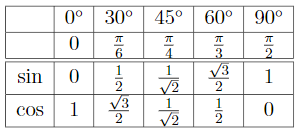
\includegraphics[width=6cm]{sincos.png} \hfill \break
                        (Sin: $\frac{\sqrt{0}}{2},\frac{\sqrt{1}}{2},\frac{\sqrt{2}}{2},\frac{\sqrt{3}}{2},\frac{\sqrt{4}}{2})$\\
        \midrule
        S   & 5.10.8&   \textbf{Trigonometrischer Pythagoras}\hfill \break
                        $sin^2(x) + cos^2(x) = 1$, für alle $x \in \mathbb{R}$ \\
        \midrule
        D   & 5.10.9&   Eine Funktion $f: \mathbb{R} \rightarrow \mathbb{R}$ oder $f: \mathbb{C} \rightarrow \mathbb{C}$ heißt: 
                        \begin{itemize}[topsep=-0.5cm]
                            \item[a)] ungerade, falls $f(-x) = -f(x)$ für alle $x \in \mathbb{R}$ bzw. $\mathbb{C}$ gilt.
                            \item[b)] gerade, falls $f(-x) = f(x)$ für alle $x \in \mathbb{R}$ bzw. $\mathbb{C}$ gilt.
                            \item[c)] periodisch mit Periode $L \in \mathbb{R}$, bzw. $\mathbb{C}$, wenn $f(x+L) = f(x)$ für alle $x \in \mathbb{R}$ bzw. $\mathbb{C}$ gilt.
                        \end{itemize} \vspace{-0cm}\\
        \midrule
        S   & 5.10.10&  Der Cosinus ist \textbf{gerade} und der Sinus ist \textbf{ungerade}. \\
        \midrule
        S   & 5.10.11&  \textbf{Eulersche Formel} \hfill \break
                        Für alle $z \in \mathbb{C}$ gilt $e^{iz} = cos(z)+sin(z)i$. \hfill \break
                        Insbesondere gilt für alle $x \in \mathbb{R}$ damit $Re(e^{ix}) = cos(x)$ und $Im(e^{ix})=sin(x)$. \\
        \midrule
        S   & 5.10.12&  Für alle $x,y \in \mathbb{R}$ gilt 
                        \begin{itemize}[topsep=-0.5cm]
                            \item[a)] $|sin(x)| \leq 1$ und $|cos(x)| \leq 1$
                            \item[b)] Additionstheoreme:
                                        \begin{itemize}[topsep=-0.5cm]
                                            \item[] $sin(x+y) = sin(x)cos(y)+sin(y)cos(x)$
                                            \item[] $cos(x+y) = cos(x)cos(y)+sin(x)sin(y)$ 
                                        \end{itemize}
                            \item[c)] Rechenregeln für verschobene Funktionen:
                                        \begin{itemize}[topsep=-0.5cm]
                                            \item[] $sin(x + \frac{\pi}{2}) = cos(x)$
                                            \item[] $sin(x + \pi) = -sin(x)$
                                            \item[] $sin(x+2\pi) = sin(x)$
                                            \item[] $cos(x + \frac{\pi}{2}) = -sin(x)$
                                            \item[] $cos(x+\pi) = -cos(x)$
                                            \item[] $cos(x+2\pi) = cos(x)$
                                            \item[] Sinus und Cosinus sind periodisch mit Periode $2\pi$      
                                        \end{itemize} \vspace{-0cm}
                        \end{itemize} \\
        \midrule
        S   & 5.10.13&  Es ist
                        \begin{itemize}[topsep=-0.5cm]
                            \item[] $sin(z) = 0 \Leftrightarrow z = k\pi$ für ein $k \in \mathbb{Z}$
                            \item[] $cos(z) = 0 \Leftrightarrow z = \frac{\pi}{2}+k\pi$ für ein $k \in \mathbb{Z}$ 
                        \end{itemize} \vspace{-0cm} \\
        \midrule
        D   & 5.10.14&  Die Funktion $tan: \mathbb{C} \textbackslash \{\frac{\pi}{2}+k\pi:k \in \mathbb{Z}\} \rightarrow \mathbb{C}$ mit \hfill \break
                        \centerline{$tan(z) = \frac{sin(z)}{cos(z)}$}
                        heißt \textbf{Tangens}. \\
        \midrule
        D   & 5.10.15&  \begin{minipage}{\linewidth}
                            \begin{itemize}
                                \item[] arcsin: $[-1,1] \rightarrow [\frac{-\pi}{2},\frac{\pi}{2}]$ (\textbf{Arcussinus})
                                \item[] arccos: $[-1,1] \rightarrow [0, \infty]$ (\textbf{Arcuscosinus})
                                \item[] arctan: $\mathbb{R} \rightarrow [\frac{-\pi}{2},\frac{\pi}{2}]$ (\textbf{Arcustangens})
                            \end{itemize}
                        \end{minipage}\\

        \bottomrule

    \end{longtable}

\pagebreak

\subsubsection{Die Polardarstellung komplexer Zahlen}

    \begin{longtable}{p{0.75cm} p{1cm} p{16cm}}
        \toprule
        D   & 5.10.17&  Es sei $Z = x + yi \in \mathbb{C} \textbackslash \{0\}$ mit $x,y \in \mathbb{R}$. Dann heißt $r:= \sqrt{x^2+y^2}$ der \textbf{Betrag}
                        von $z$ und der Winkel $\phi$, der zwischen $z$ und der positiven reellen Achse eingeschlossen wird das \textbf{Argument} von $z$.
                        Beide Werte zusammen $(r,\phi)$ zusammen sind die \textbf{Polarkoordinaten} von $z$.\\
        \midrule
        B   & 5.10.17&  Argument im Intervall $(-\pi, \pi]$ oder $[0, 2\pi)$ um Eindeutigkeit zu garantieren. \\
        \midrule
        B   & 5.10.18&  Argument: $(-\pi, \pi)$ $\rightarrow$ Umrechnung von Komplex zu Polarkoordinaten
                        \begin{itemize}[topsep=-0.5cm]
                            \item[] $x = r~cos(\phi)$
                            \item[] $y= r~sin(\phi)$ 
                            \item[] $r = \sqrt{x^2+y^2}$
                            \item[] $\phi = \begin{cases}
                                            arctan\frac{y}{x}, & x > 0 \\
                                            arctan\frac{y}{x}+\pi, & x<0 \text{ und } y \geq 0 \\
                                            arctan\frac{y}{x}-\pi, & x<0 \text{ und } y < 0 \\
                                            \frac{\pi}{2}, & x=0 \text{ und } y > 0 \\
                                            -\frac{\pi}{2}, & x=0 \text{ und } y < 0 \\
                                            \end{cases}$   
                        \end{itemize}\\
        \midrule
        S   & 5.10.19&  Es seien $z=re^{i\phi}$, $w=se^{i\psi} \in \mathbb{C} \textbackslash \{0\}$ mit Polarkoordinaten $(r,\phi)$, bzw. $(s,\phi)$
                        gegeben. Dann hat $z \cdot w$ die Polarkoordinaten $(rs, \phi + \psi)$ und $\frac{z}{w}$ die Polarkoordinaten
                        $(\frac{r}{s}, \phi - \psi)$. \\
        \midrule
        BSP & 5.10.20&  Wir berechnen $(1+i)^{2001}$. \hfill \break
                        $(1+i)^{2001} = (\sqrt{2}e^{i\frac{\pi}{4}})^{2011} = \sqrt{2}^{2011} e^{i2011\cdot \frac{\pi}{4}} =
                        \sqrt{2} \cdot 2^{1005} e^{i(2008+3)\frac{\pi}{4}} = \sqrt{2} \cdot 2^{1005} e^{i502\pi}e^{i\frac{3\pi}{4}}= 
                        2^{1005} \cdot \sqrt{2} e^{i\frac{3\pi}{4}} = 2^{1005} (-1+i)$ ($e^{i502\pi} =1$)\\
        \bottomrule

    \end{longtable}

\subsubsection{Hyperbolische Funktionen}
      
    \begin{longtable}{p{0.75cm} p{1cm} p{16cm}}
        \toprule

        D   & 5.10.22&  \begin{minipage}{\linewidth}
                            \begin{itemize}
                                \item[] $sinh(z) := \frac{e^z-e^{-z}}{2}$, $z \in \mathbb{C}$ (\textbf{Sinus hyperbolicus})
                                \item[] $cosh(z) := \frac{e^z+e^{-z}}{2}$, $z \in \mathbb{C}$ (\textbf{Cosinus hyperbolicus})
                                \item[] $tanh(z) := \frac{sinh(z)}{cosh(z)}$, $z \in \mathbb{C} \textbackslash \{(k\pi + \frac{\pi}{2}i: k \in \mathbb{Z})\}$ (\textbf{Tangens hyperbolicus})
                            \end{itemize}
                        \end{minipage} \\

        \bottomrule

    \end{longtable}

\pagebreak

\section{Analysis - Teil II: Differential- und Integralrechnung}
\subsection{Differenzierbarkeit von Funktionen in einer Variablen}
\subsubsection{Der Ableitungsbegriff}

    \begin{longtable}{p{0.75cm} p{1cm} p{16cm}}
        \toprule

        D   & 6.1.1 &   Für ganzes Kapitel gilt: $I \subseteq \mathbb{R}$ als Intervall.
                        \begin{itemize}[topsep=-0.5cm]
                            \item[a)] Es sei $x_0 \in I$. Eine Funktion $f: I \rightarrow \mathbb{R}$ heißt differenzierbar in $x_0$, wenn der Grenzwert 
                                        \centerline{$lim_{x \rightarrow x_0} \frac{f(x)-f(x_0)}{x-x_0}$}
                                        in $\mathbb{R}$ existiert. In diesem Fall heißt dieser Grenzwert die \textbf{Ableitung} von $f$ in $x_0$ und wird 
                                        mit \textbf{$f'(x_0)$} bezeichnet.
                            \item[b)] Eine Funktion $f: I \rightarrow \mathbb{R}$ heißt \textbf{differenzierbar} auf $I$, falls sie in allen Punkten
                                        $x_0 \in I$ differenzierbar ist. In diesem Fall wird $x \rightarrow f'(x)$  für $x \in I$ eine Funktion 
                                        $f': I \rightarrow \mathbb{R}$ definiert. Diese Funktion heißt die \textbf{Ableitung} oder auch 
                                        \textbf{Ableitungsfunktion} von $f$ auf $I$.
                        \end{itemize} \vspace{-0cm} \\
        \midrule
        B   & 6.1.1 &   Der Grenzwert in 6.1.1 existiert genau dann, wenn der Grenzwert $lim_{h \rightarrow 0} \frac{f(_x0 + h)-f(x_0)}{h}$
                        existiert. Die Werte stimmen dann überein. Je nach Situation den einen oder anderen verwenden. \\
        \midrule
        BSP & 6.1.3 &   $f(x) = c$ $\rightarrow$ $lim_{x \rightarrow x_0} \frac{f(x)-f(x_0)}{x-x_0} = lim_{x \rightarrow x_0}
                        \frac{0}{x-x_0} = 0$ (Ableitung konstanter Funktionen ist 0) \\
        \midrule
        S   & 6.1.4 &   Es sei $f: I \rightarrow \mathbb{R}$ in $x_0 \in I$ differenzierbar. Dann ist $f$ \textbf{stetig} in $x_0$. \hfill \break
                        (Jede differenzierbare Funktion ist stetig) \\
        \midrule
        B   & 6.1.6 &   Die Exponentialfunktion ist auf $\mathbb{R}$ differenzierbar und es gilt $E'(x) = e^x = E(x)$. \\
        \midrule
        BSP & 6.1.6 &   $f(x) = x^2$, $x \in \mathbb{R}$ \hfill \break
                        Für jedes $x_0 \in \mathbb{R}$ gilt: \hfill \break
                        \centerline{$\frac{f(x)-f(x_0)}{x-x_0}= \frac{x^2-x_0^2}{x-x_0} = \frac{(x-x_0)(x+x_0)}{x-x_0} = x+x_0$}
                        Daraus folgt: \hfill \break
                        \centerline{$lim_{x \rightarrow x_0} \frac{f(x)-f(x_0)}{x-x_0} = lim_{x \rightarrow x_0}(x+x_0) = 2x_0$}
                        Damit ist $f$ auf $\mathbb{R}$ differenzierbar und es gilt $f'(x) = 2x$, $x \in \mathbb{R}$. \\
        \midrule
        S   & 6.1.7 &   Eine Funktion $f: I \rightarrow \mathbb{R}$ ist in $x_0 \in I$ genau dann \textbf{differenzierbar} mit $f'(x_0)=a$
                        , wenn \hfill \break
                        \centerline{$f(x) = f(x_0) + a(x-x_0)+r(x)$, $x \in I$}
                        ist und für die Funktion $r: I \rightarrow \mathbb{R}$ gilt \hfill \break
                        \centerline{$lim_{x \rightarrow x_0}\frac{|r(x)|}{|x-x_0|} = 0$}. \\
        
        \bottomrule

    \end{longtable}

\subsubsection{Ableitungsregeln}

    \begin{longtable}{p{0.75cm} p{1cm} p{16cm}}
        \toprule

        S   & 6.1.9 &   Es seien $f,g: I \rightarrow \mathbb{R}$ in $x_0 \in I$ differenzierbar und $\alpha,\beta \in \mathbb{R}$. Dann gilt
                        \begin{itemize}[topsep=-0.5cm]
                            \item[a)] $\alpha f +\beta g$ ist in $x_0$ differenzierbar und \hfill \break
                                        \centerline{$(\alpha f + \beta g)'(x_0) = \alpha f'(x_0) + \beta g'(x_0)$. \textbf{(Linearität)}}
                            \item[b)] $fg$ ist differenzierbar in $x_0$ und \hfill \break
                                        \centerline{$ (fg)'(x_0)=f'(x_0)g(x_0) + f(x_0)g'(x_0)$. (\textbf{Produktregel})}
                            \item[c)] Ist $g(x_0) \neq 0$, so existiert ein Intervall $J \subseteq I$ mit $x_0 \in J$ und $g(x) \neq 0$ für
                                        alle $x \in J$. Außerdem ist die Funktion $\frac{f}{g}: J \rightarrow \mathbb{R}$ 
                                        differenziber und es gilt \hfill \break
                                        \centerline{$(\frac{f}{g})'(x_0)= \frac{f'(x_0)g(x_0)-f(x_0)g'(x_0)}{(g(x_0))^2}$. (\textbf{Quotientenregel})} 
                        \end{itemize} \vspace{-0cm} \\
        \midrule
        S   & 6.1.10&   \textbf{Kettenregel} \hfill \break
                        Es seien $I, J \subseteq \mathbb{R}$ Intervalle und $g: I \rightarrow J$ sei differenzierbar in $x_0 \in I$.
                        Weiter sei $f:J \rightarrow \mathbb{R}$ differenzierbar in $y_0 = g(x_0)$. Dann ist auch die Funktion
                        $f \circ g: I \rightarrow \mathbb{R}$ differenzierbar in $x_0$ und es gilt \hfill \break
                        \centerline{$(f\circ g)'x_0 = f'(g(x_0)) \cdot g'(x_0)$.} \\
        \midrule
        BSP & 6.1.11&   $a > 0$, $\phi(x):= a^x$, $x \in \mathbb{R}$ (allgemein) \hfill \break
                        $\phi(x) = e^{x\cdot ln(a)}$: $f(x) = e^y$ und $g(x) = x\cdot ln(a)$ $\rightarrow$ $\phi = f\circ g$ \hfill \break
                        $\phi' = f'(g(x))g'(x) = e^{g(x)}ln(a) = e^{x\cdot ln(a)}ln(a) = a^xln(a)$ \\
        \midrule
        S   & 6.1.12&   Es sei $f \in C(I)$ streng monoton und $x_0 \in I$ differenzierbar mit \textbf{$f'(x_0) \neq 0$}. Dann existiert die
                        \textbf{Umkehrfunktion} $f^{-1}: f(I) \rightarrow \mathbb{R}$, diese ist differenzierbar in $y_0 = f(x_0)$ und es gilt \hfill \break
                        \centerline{$(f^{-1})'(y_0) = \frac{1}{f'(x_0)} $} \\
        \midrule
        B   & 6.1.12&   Wichtig: $f'(x_0) \neq 0$ als Voraussetzung! \\
        \midrule
        BSP & 6.1.14&   \textbf{Ableitung des ln} \hfill \break
                        $f(x) = e^x$, $f^{-1}(x) = ln(x)$ \hfill \break
                        $(ln)'(y) = (f^{-1})'(y) = \frac{1}{f'(x)} = \frac{1}{e^x} = \frac{1}{e^{ln(y)}} = \frac{1}{y}$, $y \in (0, \infty)$ \\
        \midrule
        S   & 6.1.15&   Es sei $f(x) = \sum^{\infty}_{n=0} a_n  x^n$ eine Potenzreihe in $\mathbb{R}$ mit Konvergenzradius $r >0$. Dann hat
                        auch die Potenzreihe $\sum^{\infty}_{n=1} na_nx^{n-1}$ den Konvergenzradius $r$, die Funktion $f$ ist in allen
                        $x \in (-r,r)$ differenzierbar und es gilt \hfill \break
                        \centerline{$f'(x) = \sum^{\infty}_{n=1} na_n x^{n-1}$, $x \in (-r,r)$}
                        (Potenzreihe im Inneren des Konvergenzgebietes summandenweise ableitbar)\\
        \midrule
        BSP & 6.1.16&   Potenzreihen von Sinus und Cosinus konvergieren auf ganz $\mathbb{R}$. \hfill \break
                        \centerline{$ sin'(x) = (\sum^{\infty}_{n=0} \frac{(-1)^n}{(2n+1)!} x^{2n+1})' = 
                        \sum^{\infty}_{n=0} \frac{(-1)^n}{(2n)!}x^{2n} = cos(x)$}
                        \centerline{$cos'(x) = -sin(x)$} \\
        \midrule
        BSP & 6.1.17&   Berechnung des Reihenwerts mithilfe von 6.1.15 \hfill \break
                        Potenzreihe $\sum^{\infty}_{n=1} nx^n$, Konvergenzradius $1$, Welche Funktion ist hier gegeben? \hfill \break
                        Für alle $x\in (-1,1)$ gilt: $\sum^{\infty}_{n=1} nx^n = x \sum^{\infty}_{n=1} nx^{n-1} =
                        x \sum^{\infty}_{n=1} (x^n)' = x(\sum^{\infty}_{n=1} x^n)'$ \hfill \break
                        Nun bis auf fehlenden ersten Summanden gleich der schon bekannten geometrische Reihe. Für $x \in (-1,1)$ gilt: \hfill \break
                        \centerline{$ \sum^{\infty}_{n=1} nx^n = x( \frac{1}{1-x} - 1)' = x \frac{-1}{(1-x)^2}(-1) = \frac{x}{(1-x)^2} $} \\
        \midrule
        B   &       &   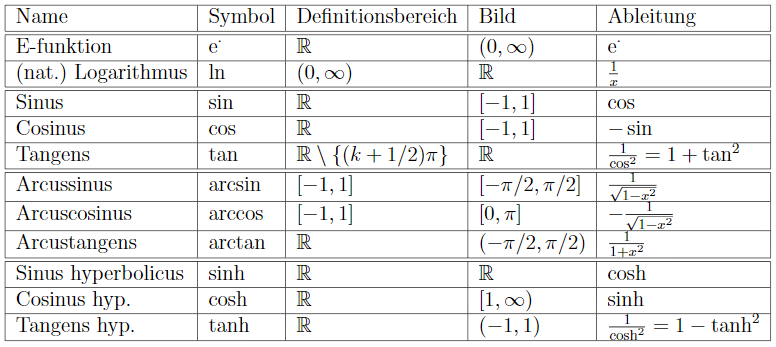
\includegraphics[width=6cm]{ableitungen.png} \\
        \bottomrule
    \end{longtable}

\subsubsection{Höhere Ableitungen}
      
    \begin{longtable}{p{0.75cm} p{1cm} p{16cm}}
        \toprule

        D   & 6.1.19&   Ist $f: I \rightarrow \mathbb{R}$ eine in $I$ differenzierbare Funktion und ist $f'$ auf $I$ stetig, so nennt man
                        $f$ \textbf{stetig differenzierbar}. Man schreibt $C^1(I) := \{ f:I \rightarrow \mathbb{R}: f$ stetig differenzierbar\} \\
        \midrule
        D   & 6.1.20&   \begin{minipage}{\linewidth}
                            \begin{itemize}
                                \item[a)] Es sei $f: I \rightarrow \mathbb{R}$ differenzierbar auf $I$, $x_0 \in I$ und $n \in \mathbb{N}$ mit
                                            $n \geq 2$. Dann heißt die Funktion $f$ in $x_0$ (bzw. auf $I$) \textbf{$n$-mal differenzierbar}
                                            falls sie auf $I$ schon $(n-1)$ differenzierbar ist und die Funktion $f^{(n-1)}$ in $x_0$
                                            (bzw. auf $I$) wieder differenzierbar ist. \hfill \break
                                            In diesem Fall heißt $f^{(n)}(x_0) = (f^{(n-1)})'(x_0)$ die \textbf{$n$-te Ableitung} von $f$ in
                                            $x_0$ bzw. $x \rightarrow f^{(n)}(x)$ die $n$-te Ableitungsfunktion von $f$ auf $I$. 
                                \item[b)] Ist die $n$-te Ableitung von $f$ auf $I$ selbst sogar wieder stetig auf $I$, so sagt man $f$ sei
                                            sei $n$-mal \textbf{stetig differenzierbar} auf $I$. Man schreibt \hfill \break
                                            \centerline{$ C^n(I) := \{ f: I \mathbb{R}: f~n$-mal stetig differenzierbar\}.}
                                \item[c)] Ist $f\in C^n(I)$ für alle $n \in \mathbb{N}$, so nennt man $f$ \textbf{beliebig oft differenzierbar}.
                                            Man verwendet dafür die Bezeichnung \hfill \break
                                            \centerline{$f \in C^{\infty}(I) := \prod_{n \in \mathbb{N}} C^n(I)$.}
                            \end{itemize}
                        \end{minipage} \\
        \midrule
        B   & 6.1.20&   Die Funktion selbst wird als nullte Ableitung definiert $f^{(0)} := f$. \\
        \bottomrule

    \end{longtable}

\pagebreak

\subsection{Eigenschaften differenzierbarer Funktionen}

    \begin{longtable}{p{0.75cm} p{1cm} p{16cm}}
        \toprule
        S   & 6.2.1 &   \textbf{Mittelwertsatz der Differenzialrechnung} \hfill \break
                        Es seien $a,b \in \mathbb{R}$ mit $a < b$ und $f \in C([a,b])$ sei differenzierbar in $(a,b)$. Dann gibt es ein
                        $\xi \in (a,b)$, so dass $\frac{f(b)-f(a)}{b-a} = f'(\xi)$, bzw. gleichbedeutend $f(b) - f(a) = f'(\xi)(b-a)$ gilt. \\
        \midrule
        B   & 6.2.1 &   Sekantensteigung der Funktion (erhalten durch $a$ und $b$) entspricht irgendwann zwischen $a$ und $b$ tatsächlich
                        der Tangentensteigung. \hfill \break
                        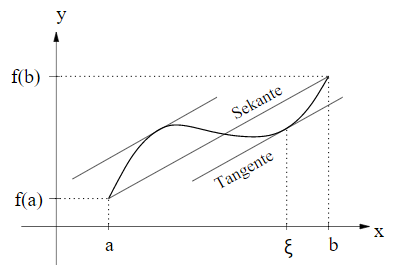
\includegraphics[width=7cm]{mws.png} \\
        \midrule
        S   & 6.2.2 &   \begin{minipage}{\linewidth}
                            \begin{itemize}
                                \item[a)] \textbf{Satz von Rolle} \hfill \break
                                            Es seien $a, b \in \mathbb{R}$ mit $a < b$ und $f \in C([a,b])$. Ist $f$ auf $(a,b)$ differenzierbar
                                            und gilt $f(a) = f(b)$, so gibt es ein $\xi \in (a,b)$ mit $f'(\xi) = 0$.
                                \item[b)] Es sei $f: I \rightarrow \mathbb{R}$ auf dem \textbf{Intervall} $I$ differenzierbar. Dann gilt
                                            \begin{itemize}[topsep=-0.5cm]
                                                \item[] Ist $f' = 0$ auf $I$, so ist $f$ auf $I$ konstant.
                                                \item[] Ist $f' > 0$ auf $I$, so ist $f$ auf $I$ streng monoton wachsend.
                                                \item[] Ist $f' < 0$ auf $I$, so ist $f$ auf $I$ streng monoton fallend.
                                                \item[] Ist $f' \geq 0$ auf $I$, so ist $f$ auf $I$ monoton wachsend.
                                                \item[] Ist $f' \leq 0$ auf $I$, so ist $f$ auf $I$ monoton fallend.
                                            \end{itemize}
                                \item[c)] Sind $f,g : I \rightarrow \mathbb{R}$ auf $I$ differenzierbare Funktionen und gilt $f' = g'$ auf $I$,
                                            so gibt es eine Konstante $c \in \mathbb{R}$, so dass $f(x) = g(x) + c$ für alle $x \in I$ gilt.
                            \end{itemize}
                        \end{minipage} \\
        \midrule
        S   & 6.2.6 &   \textbf{Satz von de l'Hospital} \hfill \break
                        Es sei $(a,b)$ ein offenes Intervall $\mathbb{R}$ ($a= - \infty$ und $b = \infty$ hier zugelassen)  und $f,g:
                        (a,b) \rightarrow \mathbb{R}$ seien differenzierbar auf $(a,b)$ mit $g'(x) \neq 0$ für alle $x \in (a,b)$. Gilt dann
                        \hfill \break
                        \centerline{$lim_{x \rightarrow a} f(x) = lim_{x \rightarrow a} g(x) = 0$ oder $lim_{x \rightarrow a} f(x) = 
                        lim_{x \rightarrow a} g(x) = \pm \infty$} 
                        und existiert der Grenzwert \hfill \break
                        \centerline{$ L := lim_{x \rightarrow a} \frac{f'(x)}{g'(x)} $} 
                        ($L = \pm \infty$ zugelassen), dann gilt \hfill \break
                        \centerline{$lim_{x \rightarrow a} \frac{f(x)}{g(x)} = L$.}\\
        \midrule
        B   & 6.2.6 &   Achtung! Alle Voraussetzungen prüfen! \\
        \midrule
        D   & 6.2.9 &   Es sei $I \subseteq \mathbb{R}$ ein offenes Intervall, $x_0 \in I$ und $f \in C^{\infty}(I)$.
                        \begin{itemize}[topsep=-0.5cm]
                            \item[a)] Die Potenzreihe \hfill \break
                                        \centerline{$\sum^{\infty}_{n=0} \frac{f^{(n)}(x_0)}{n!}(x-x_0)^n$}
                                        heißt \textbf{Taylorreihe} von $f$ um $x_0$.
                            \item[b)] Für jedes $k \in \mathbb{N}$ heißt das Polynom \hfill \break
                                        \centerline{$T_{k,f}(x;x_0) := \sum^{k}_{n=0} \frac{f^{(n)}(x_0)}{n!}(x-x_0)^n$}
                                        das \textbf{Taylorpolynom k-ten Grades} von $f$ in $x_0$.
                        \end{itemize} \vspace{-0cm}  \\
        \midrule
        BSP & 6.2.10&   Taylorpolynom $k$-ten Grades ist anschaulich die bestmögliche Approximation an die Funktion $f$ \\
        \midrule
        S   & 6.2.12&   \textbf{Satz von Taylor} \hfill \break
                        Es seien $I \subseteq \mathbb{R}$ ein offenes Intervall, $x,x_0 \in I$ und für ein $k \in \mathbb{N_0}$ sei $f:I \rightarrow \mathbb{R}$
                        eine $k+1$-mal differenzierbare Funktion. Dann gibt es ein $\xi$ zwischen $x$ und $x_0$, so dass gilt \hfill \break
                        \centerline{$ f(x) = T_{k,f}(x;x_0) + \frac{f^{k+1}(\xi)}{(k+1)!} (x-x_0)^{k+1} $} 
                        (Vorne Annäherung, hinten Fehlerterm - Abschätzung wie gut die Taylorreihe zu Funktion passt) \\
        \midrule
        B   & 6.2.12&   \begin{itemize}[topsep=-0.5cm]
                            \item[a)] Taylor für $k=0$ ist Mittelwertsatz.
                            \item[b)] Der Fehlerterm \hfill \break
                                        \centerline{$ R_{k,f}(x;x_0) := \frac{f^{k+1}(\xi)}{(k+1)!}(x-x_0)^{k+1}$,}
                                        der die Differenz zwischen $f(x)$ und der Näherung durch das Taylorpolynom $k$-ten Grades beschreibt,
                                        wird auch als Restglied bezeichnet.
                        \end{itemize} \vspace{-0cm} \\

        \bottomrule

    \end{longtable}

\subsection{Extremwerte}

    \begin{longtable}{p{0.75cm} p{1cm} p{16cm}}
        \toprule

        D   & 6.3.1 &   Es sei $D \subseteq \mathbb{R}$ und $f: D \rightarrow \mathbb{R}$ eine Funktion.
                        \begin{itemize}[topsep=-0.5cm]
                            \item[a)] Man sagt, dass $f$ in $x_0 \in D$ ein \textbf{globales Maximum} (bzw. Minimum) hat, falls $f(x) \leq f(x_0)$
                                        (bzw. $f(x) \geq f(x_=)$) für alle $x \in D$ gilt.
                            \item[b)] $f$ hat in $x_0 \in D$ ein \textbf{relatives Maximum} (bzw. Minimum), falls ein $\delta > 0$ existiert, so dass $f(x) \leq f(x_0)$
                                        (bzw. $f(x) \geq f(x_0)$) für alle $x \in D$ mit $|x-x_0| < \delta$ gilt.
                            \item[c)] Allgemein spricht man von einem globalen bzw. relativen \textbf{Extremum} in $x_0$ wenn $f$ dort ein entsprechendes
                                        Maximum oder Minimum hat.
                        \end{itemize} \vspace{-0cm} \\
        \midrule
        S   & 6.3.3 &   Es sei $f: I \rightarrow \mathbb{R}$ differenzierbar in $x_0 \in I$. Ist $x_0$ ein innerer Punkt von $I$ und hat $f$ in $x_0$
                        ein relatives Extremum, so gilt $f'(x_0) = 0$. \\
        \midrule
        B   & 6.3.3 &   Innerer Punkt von D: Kein Randpunkt, möglich Kugel um den Punkt zu legen \hfill \break
                        Warnung: $x_0$ innerer Punkt ist wesentlich \hfill \break
                        Warnung: Umkehrung des Satzes gilt nicht (Kann auch Sattelpunkt sein, nicht unbedingt Extremum) \\
        \midrule
        S   & 6.3.5 &   Es sei $I \subseteq \mathbb{R}$ ein Intervall, $x_0 \in I^{\circ}$ und $f \in C^n(I)$ für ein $n \geq 2$. Weiter gelte
                        $f'(x_0) = f''(x_0) = \dots = f^{n-1}(x_0) = 0$, aber $f^{(n)}(x_0) \neq 0$. Ist nun $n$ ungerade, so hat $f$ in $x_0$ kein
                        Extremum, ist $n$ gerade, so liegt in $x_0$ ein Extremum vor, und zwar falls $f^{(n)}(x_0) > 0$ ein \textbf{Minimum} und falls
                        $f^{(n)}(x_0) < 0$ ein \textbf{Maximum}. \\
        \bottomrule

    \end{longtable}

\subsection{Differenzieren von Funktionen mehrerer Variablen - Partielle Ableitung}

    \begin{longtable}{p{0.75cm} p{1cm} p{16cm}}
        \toprule

        D   & 6.4.1 &   Es sei $G \subseteq \mathbb{R}^d$ offen, $f: G \rightarrow \mathbb{R}^p$ eine Funktion, $x_0 \in G$ und $v \in \mathbb{R}^d 
                        \textbackslash \{0\}$. Existiert der Grenzwert \hfill \break
                        \centerline{$ (\partial_v f) (x_0) := lim_{h \rightarrow 0} \frac{f(x_0 +hv) - f(x_0)}{h}$,}
                        so heißt $f$ in $x_0$ in Richtung $v$ differenzierbar und $(\partial_v f)(x_0)$ die \textbf{Richtungsableitung}
                        von $f$ in $x_0$ in Richtung $v$. (Betrachtung der Funktionswerte entlang einer Geraden im Raum) \\
        \midrule
        B   & 6.4.1 &   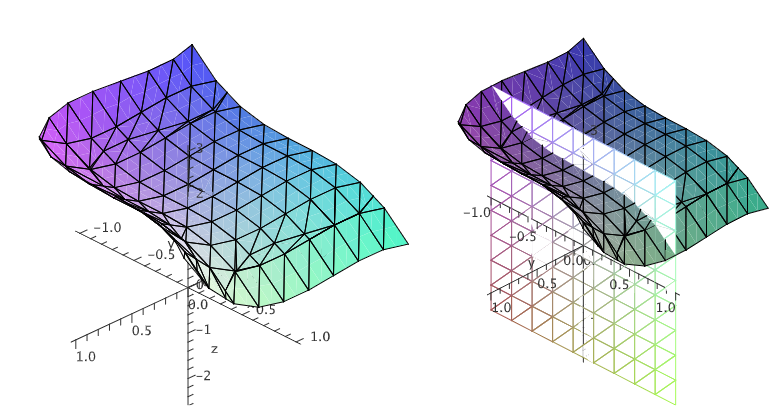
\includegraphics[width=8cm]{partAbl.png} \\
        \midrule
        D   & 6.4.3 &   Es seien $G \subseteq \mathbb{R}^d$ offen, $f: G \rightarrow \mathbb{R}^p$ eine Funktion und $\{ e_1,e_2,\dots,e_d \}$ die
                        \textbf{Standardbasis} des $\mathbb{R}^d$.
                        \begin{itemize}[topsep=-0.5cm]
                            \item[a)] Existieren in einem $x_0 \in G$ die Richtungsableitungen von $f$ in alle Richtungen $e_1, e_2, \dots e_d$, so heißt
                                        $f$ in $x_0$ \textbf{partiell differenzierbar}. Man schreibt dann für $j =1,2,\dots,d$ auch \hfill \break
                                        \centerline{$ \partial_j f(x_0) := \frac{\partial f}{\partial x_j} (x_0) := f_{x_j}(x_0) := (\partial_{e_j}f) (x_0)$}
                                        für die \textbf{partielle Ableitung von f in $x_0$ nach der j-ten Koordinate}.
                            \item[b)] Ist $f$ in allen $x_0 \in G$ partiell differenzierbar, so sagt man $f$ ist in $G$ partiell differenzierbar und schreibt
                                        $\partial_j f = \frac{\partial f}{\partial x_j} = f_{x_j} : G \rightarrow \mathbb{R}^p$ für die \textbf{partielle
                                        Ableitungs(-funktion)}
                            \item[c)] Ist $f$ in $G$ partiell differenzierbar und sind sämtliche partielle Ableitungen $\partial_1 f, \partial_2 f, \dots,
                                        \partial_d f: G \rightarrow \mathbb{R}^p$ stetig, so nennt man $f$ \textbf{stetig partiell differenzierbar} in $G$.
                        \end{itemize} \vspace{-0cm} \\  \\
        \midrule
        B   & 6.4.3 &   Berechnung Ableitung: Alle anderen Variablen werden als konstante Parameter behandelt \\
        \midrule
        BSP & 6.4.7 &   $f: \mathbb{R}^3 \rightarrow \mathbb{R}$ mit $f(x,y,z) = xe^{xz+y^2}$: 
                        \begin{itemize}[topsep=-0.5cm]
                            \item[] $\partial_1 f(x,y,z) = e^{xz+y^2} + xe^{xz+y^2} \cdot z$ 
                            \item[] $\partial_2 f(x,y,z) = xe^{xz+y^2} \cdot 2y$
                            \item[] $\partial_3 f(x,y,z) = xe^{xz+y^2} \cdot x$
                        \end{itemize} \vspace{-0cm}\\
        \midrule
        S   & 6.4.8 &   Ist $G \subseteq \mathbb{R}^d$ offen, $f: G \rightarrow \mathbb{R}^p$ eine Funktion und $x_0 \in G$, so ist $f$ in $x_0$
                        genau dann partiell differenzierbar, wenn alle Koordinatenfunktionen $f_1, f_2, \dots, f_p : G\rightarrow \mathbb{R}$ in $x_0$
                        partiell differenzierbar sind. In diesem Fall gilt \hfill \break
                        \centerline{$ \partial_j f(x_0) = (\partial_1 f_1(x_0), \partial_j f_2(x_0), \dots, \partial_j f_p(x_0) )^T$} \\
        \midrule
        D   & 6.1.10&   Es sei $G \subseteq \mathbb{R}^d$ offen und $f: G \rightarrow \mathbb{R}^p$ in $x_0 \in G$ partiell differenzierbar. 
                        Die $p~x~d$-Matrix aller partiellen Ableitungen \hfill \break
                        \centerline{$ J_f(x_0) :=   \begin{pmatrix}
                                                    \partial_1 f_1(x_0) & \partial_2 f_1(x_0) & \dots & \partial_d f_1(x_0) \\
                                                    \partial_1 f_2(x_0) & \partial_2 f_2(x_0) & \dots & \partial_d f_2(x_0) \\
                                                    \dots & \dots & \dots & \dots \\
                                                    \partial_1 f_p(x_0) & \partial_2 f_p(x_0) & \dots & \partial_d f_p(x_0) \\
                                                    \end{pmatrix}$} 
                        heißt \textbf{Jakobi-Matrix} von $f$. \hfill \break
                        Im Spezialfall $p=1$ nennt man die $1~x~d$-Matrix, d.h. den $\mathbb{R}^d$-Zeilenvektor \hfill \break
                        \centerline{$\nabla f(x_0 := J_f(x_0)) = (\partial_1 f(x_0), \partial_2f(x_0), \dots, \partial_df(x_0))$}
                        den \textbf{Gradient} von $f$. \\
        \midrule
        B   & 6.1.10&   Es gilt $J_f(x)=    \begin{pmatrix}
                                            \nabla(f_1(x)) \\
                                            \nabla(f_2(x)) \\
                                            \dots \\
                                            \nabla(f_p(x)) \\
                                            \end{pmatrix}$ \\
        \midrule
        B   & 6.1.10&   Bedeutung Gradient: Falls $f$ glatt genug ist gibt der Vektor $\nabla f(x_0)$ die Richtung, in der der Graph von $f$ an der Stelle
                        $x_0$ am stärksten ansteigt und seine Länge entspricht dieser maximalen Steigung. (Basis für Optimierungsverfahren) \\
        \midrule
        D   & 6.4.13&   Es seien $G \subseteq \mathbb{R}^d$, $n \in \mathbb{N}$ mit $n \geq 2$, $x_0 \in G$ und $f: G \rightarrow \mathbb{R}^p$ eine Funktion.
                        Diese nennt man $n$-mal (stetig) partiell differenzierbar in $x_0$, wenn sie schon $(n-1)$-mal (stetig) partiell differenzierbar
                        auf $G$ ist und alle $(n-1)$-ten partiellen Ableitungen in $x_0$ wieder (stetig) partiell differenzierbar sind.  \hfill \break
                        Notation: $\partial_1 \partial_3 \partial_1$ (Reihenfolge meist egal, wenn nicht von innen nach außen) \\
        \midrule
        BSP & 6.4.14&   $f: \mathbb{R}^2 \rightarrow \mathbb{R}$ mit $f(x,y) = x^3 y + x e^y$ \hfill \break
                        Ableitungen erster Ordnung: \hfill \break
                        \centerline{$ \partial_1f(x,y) = 3x^2y + e^y$ und $\partial_2f(x,y) = x^3 + xe^y$}
                        Ableitungen zweiter Ordnung: \hfill \break
                        \centerline{$\partial_1^2 f(x,y) =6xy$ \hspace{1cm} $\partial_1 \partial_2f(x,y) = 3x^2 + e^y $}
                        \centerline{$ \partial_2 \partial_1 f(x,y) = 3x^2 + e^y$ \hspace{1cm} $\partial_2^2f(x,y) = xe^y$} 
                        Man beobachtet, dass das Ergebnis nicht von der Reihenfolge der Ableitungen abhängig sind. \\
        \midrule
        S   & 6.4.15&   \textbf{Satz von Schwarz} \hfill \break
                        Ist $G \subseteq \mathbb{R}^d$ offen und $f: G \rightarrow \mathbb{R}^p$ eine $n$-mal stetig partiell differenzierbare Funktion,
                        so ist die Reihenfolge der partiellen Ableitungen bis zur Ordnung $n$ vertauschbar. \hfill \break
                        (Sind die partiellen Ableitungen nicht stetig, gilt der Satz nicht.)\\ 
        \bottomrule

    \end{longtable}

\pagebreak

\subsection{Differenzieren von Funktionen mehrerer Variablen - Totale Differenzierbarkeit}

    \begin{longtable}{p{0.75cm} p{1cm} p{16cm}}
        \toprule

        D   & 6.5.1 &   Es sei $G \subseteq \mathbb{R}^d$ offen und $x_0 \in G$. Eine Funktion $f: G \rightarrow \mathbb{R}^p$ heißt
                        \textbf{(total) differenzierbar} in $x_0$, wenn es eine lineare Abbildung $\Phi: \mathbb{R}^d \rightarrow \mathbb{R}^p$
                        gibt, so dass gilt \hfill \break
                        \centerline{$ f(x) = f(x_0) * \Phi(x-x_0) + r(x)$, $x \in G$}
                        mit einer Funktion $r: G \rightarrow \mathbb{R}^p$ die \hfill \break
                        \centerline{$ lim_{x \rightarrow x_0} \frac{||r(x)||}{||x-x_0||} = 0 $}
                        erfüllt. \hfill \break
                        Die lineare Abbildung $Df(x_0) := \Phi$ heißt dann \textbf{(totale) Ableitung} von $f$ in $x_0$. Ist $f$ in allen
                        $x_0 \in G$ total differenzierbar, so nennt man die Funktion $Df: G \rightarrow \mathcal{L}(\mathbb{R}^d, \mathbb{R}^p)$
                        die \textbf{Ableitung(sfunktion)} von $f$. \\
        \midrule
        B   & 6.5.4 &   Ableitung einer linearen Abbildung $\Phi: \mathbb{R}^d \rightarrow \mathbb{R}^p$ ist in jedem Punkt die Abbildung $\Phi$ selbst \\
        \midrule
        S   & 6.5.6 &   Ist $G \subseteq \mathbb{R}^d$ offen und $f: G\rightarrow \mathbb{R}^p$ in $x_0 \in G$ total differenzierbar, so ist $f$ auch
                        stetig in $x_0$. \\
        \midrule
        S   & 6.5.7 &   Es sei $G \subseteq \mathbb{R}^d$ offen, $f: G \rightarrow \mathbb{R}^p$ eine in $x_0 \in G$ total differenzierbare Funktion und
                        $v \in \mathbb{R}^d \textbackslash \{0\}$. Dann existiert in $x_0$ die Richtungsableitung von $f$ in Richtung $v$ und es gilt \hfill \break
                        \centerline{$ (\partial_vf)(x_0) = Df(x_0)(v)$.} \\
        \midrule
        S   & 6.5.8 &   Es sei $G \subseteq \mathbb{R}^d$ offen, $x_0 \in G$ und $f: G \rightarrow \mathbb{R}^p$ eine Funktion. Ist $f$ in $x_0$ total
                        differenzierbar, so ist $f$ in $x_0$ auch partiell differenzierbar und die Abbildungsmatrix von $Df(x_0)$ bezüglich der Standardbasen
                        von $\mathbb{R}^d$ bzw. $\mathbb{R}^p$ ist die Jakobi-Matrix $J_f(x_0)$. \\
        \midrule
        B   & 6.5.8 &   Die Umkehrung dieses Satzes ist falsch. \\
        \midrule
        S   & 6.5.10&   Ist $G \subseteq \mathbb{R}^d$ offen und $f: G\rightarrow \mathbb{R}^p$ in $x_0 \in G$ total differenzierbar, so gilt für jedes
                        $ v \in \mathbb{R}^d \textbackslash \{0\}$ \hfill \break
                        \centerline{$ \partial_vf(x_0) = J_f(x_0)v $.} \\
        \midrule
        S   & 6.5.12&   Ist $G \subseteq \mathbb{R}^d$ offen und $f: G\rightarrow \mathbb{R}^p$ in $x_0 \in G$ stetig partiell differenzierbar, so ist
                        $f$ in $x_0$ sogar total differenzierbar. \\
        \midrule
        B   & 6.5.12&   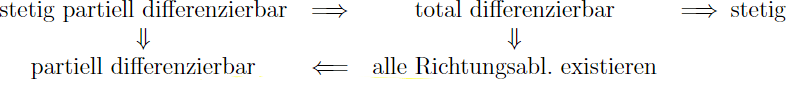
\includegraphics[width=8cm]{abspar.png} \\
        \midrule
        S   & 6.5.13&   \textbf{Kettenregel} \hfill \break
                        Es seien $G \subseteq \mathbb{R}^d$ und $H \subseteq \mathbb{R}^p$ offen, sowie $g : G\rightarrow \mathbb{R}^p$ mit $g(G) \subseteq H$
                        und $f: H \rightarrow \mathbb{R}^q$ Funktionen, so dass $g$ in $x_0 \in G$ und $f$ in $g(x_0)$ total differenzierbar sind. Dann ist 
                        auch die Funktion $f \circ g : G \rightarrow \mathbb{R}^q$ in $x_0$ total differenzierbar und es gilt \hfill \break
                        \centerline{$ D(f\circ g)(x_0) = Df(g(x_0)) \cdot Dg(x_0) $.} 
                        (Enthält Matrixmultiplikation)\\
        \midrule
        S   & 6.5.16&   \textbf{Mittelwertsatz} \hfill \break
                        Es sei $G \subseteq \mathbb{R}^d$ offen und $f : G \rightarrow \mathbb{R}$ eine total differenzierbare Funktion. Sind 
                        $a,b \in G$ so gewählt, dass $\bar{ab} \subseteq G$ , so gibt es ein $\xi \in \bar{ab}$ mit \hfill \break
                        \centerline{$f(b) - f(a) = \nabla f(\xi)(b-a)$} \\
        \midrule
        B   & 6.5.16&   $\bar{ab} := \{a+\lambda(b-a):\lambda \in [0,1]\}$: Verbindungsstrecke von $a$ nach $b$ \\
        \midrule
        D   & 6.5.17&   Eine Menge $M \subseteq \mathbb{R}^d$ heißt \textbf{konvex}, wenn für alle $a,b \in M$ auch $\bar{ab} \subseteq M$ gilt. \\
        \midrule
        S   & 6.5.18&   \textbf{Schrankensatz} \hfill \break
                        Es sei $G \subseteq \mathbb{R}^d$ offen und konvex, sowie $f: G \rightarrow \mathbb{R}$ total differenzierbar. Gibt es ein
                        $L \geq 0$ mit $||\nabla f(x)||_2 \leq L$ für alle $x \in G$, so gilt \hfill \break
                        \centerline{$ |f(x) - f(y)| \leq L||x-y||_2 $, für alle $x,y \in G$}
                        d.h. $f$ ist \textbf{Lipschitz-stetig} auf $G$. \\
        \midrule
        D   & 6.5.20&   Es sei $G \subseteq \mathbb{R}^d$ offen und $f: G \rightarrow \mathbb{R}$ in $x_0 \in G$ zweimal partiell differenzierbar.
                        Dann heißt die Matrix der zweiten partiellen Ableitungen \hfill \break
                        \centerline{$ H_f(x_0) := (\partial_j \partial_k f(x_0))_{j,k = 1,\dots,d} $}
                        \textbf{Hesse-Matrix} von $f$ in $x_0$. \\
        \midrule
        B   & 6.5.20&   Hesse-Matrix ist immer eine quadratische Matrix. \hfill \break
                        Sogar symmetrisch, falls $f$ stetig partiell differenzierbar in $x_0$ ist \hfill \break
                        Es gilt $H_f(x_0) = J_{(\nabla f)^T}(x_0)$  \\
        \midrule
        D   & 6.5.22&   \textbf{Satz von Taylor} \hfill \break
                        Den Ausdruck \hfill \break
                        \centerline{$ T_{1,f}(x;x_0) := f(x_0) + \nabla f(x_0)(x-x_0) $}
                        bezeichnen wir wieder als das \textbf{Taylorpolynom} ersten Grades von $f$ in $x_0$. \\
        \midrule
        S   & 6.5.22&   \textbf{Satz von Taylor} \hfill \break
                        Es sei $G \subseteq \mathbb{R}^d$ eine offene und konvexe Menge und $f: G \rightarrow \mathbb{R}$ sei zweimal
                        stetig partiell differenzierbar (damit auch 2x total differenzierbar) in $G$. Zu jeder Wahl von
                        $x_0, x \in G$ gibt es dann ein $\xi \in \bar{x_0x}$ mit \hfill \break
                        \centerline{$ f(x) = f(x_0) + \nabla f(x_0)(x-x_0) + \frac{1}{2} (x-x_0)^T H_f(\xi)(x-x_0)$.} \\
        \bottomrule

    \end{longtable}

\subsection{Extremwertprobleme in mehreren Variablen}

    \begin{longtable}{p{0.75cm} p{1cm} p{16cm}}
        \toprule

        D   & 6.6.1 &   Es sei $G \subseteq \mathbb{R}^d$ und $f: G \rightarrow \mathbb{R}$.
                        \begin{itemize}[topsep=-0.5cm]
                            \item[a)] Man sagt, dass $f$ in $x_0 \in G$ ein globales Maximum (bzw. Minimum) hat, falls  $f(x) \leq f(x_0)$
                                        (bzw. $f(x) \geq f(x_0)$) für alle $x \in G$ gilt.
                            \item[b)] $f$ hat in $x_0 \in G$ ein relatives Maximum (bzw. Minimum), falls ein $\delta > 0$ existiert, so dass
                                        $f(x) \leq f(x_0)$ (bzw. $f(x) \geq f(x_0)$) für alle $x \in G$ mit $||x-x_0|| < \delta$ gilt.
                            \item[c)] Allgemein spricht man von einem globalen bzw. relativen Extremum in $x_0$, wenn $f$ dort ein entsprechendes
                                        Maximum oder Minimum hat.  
                        \end{itemize} \vspace{-0cm} \\ 
        \midrule
        S   & 6.6.2 &   Es sei $G \subseteq \mathbb{R}^d$ und $x_0$ ein innerer Punkt von $G$, sowie $f: G \rightarrow \mathbb{R}$ total
                        differenzierbar in $x_0$. Hat $f$ in $x_0$ ein relatives Extremum, so gilt $\nabla f(x_0) = 0$. \\
        \midrule
        S   & 6.6.3 &   Es sei $G \subseteq \mathbb{R}^d$ offen, $f: G \rightarrow \mathbb{R}$ zweimal stetig partiell differenzierbar und für
                        $x_0 \in G$ gelte $\nabla f(x_0) = 0$. Ist dann die Hesse-Matrix $H_f(x_0)$ 
                        \begin{itemize}[topsep=-0.5cm]
                            \item[a)] \textit{positiv definit}, so hat $f$ in $x_0$ ein relatives Minimum
                            \item[b)] \textit{negativ definit}, so hat $f$ in $x_0$ ein relatives Maximum
                            \item[c)] \textit{indefinit}, so hat $f$ in $x_0$ kein relatives Extremum
                        \end{itemize} \vspace{-0cm} \\
        \bottomrule

    \end{longtable}

\pagebreak

\subsection{Integration in $\mathbb{R}$}
\subsubsection{Definition des bestimmten Integrals}

    \begin{longtable}{p{0.75cm} p{1cm} p{16cm}}
        \toprule

        D   & 6.7.1 &   Es seien $a,b \in \mathbb{R}$ mit $a < b$. Eine endliche Menge $Z:= \{ x_0, x_1, \dots, x_n \} \subseteq [a,b]$ heißt
                        \textbf{Zerlegung} des Intervalls $[a,b]$, wenn gilt $a = x_0 < x_1 < \dots < x_{n-1} < x_n = b$. \hfill \break
                        Für eine solche Zerlegung und eine gegebene beschränkte Funktion $f: [a,b] \rightarrow \mathbb{R}$ setzen wir nun
                        für jedes $j = 1,\dots,n$ \hfill \break
                        \centerline{$ I_j := [x_{j-1},x_j], |I_j| := x_j - x_{j-1}, m_j := inf~f(I_j), M_j := sup~f(I_j)$} \\
        \midrule
        D   & 6.7.2 &   Es seien $a,b \in \mathbb{R}$ mit $a < b$, $Z = \{ x_0, \dots, x_n\}$ eine Zerlegung von $[a,b]$ und $f:[a,b]\rightarrow \mathbb{R}$
                        beschränkt. Dann heißt der Wert 
                        \begin{itemize}[topsep=-0.5cm]
                            \item[] $\underline{s}_f(Z) := \sum^{n}_{j=1} m_j |I_j|$ die \textbf{Untersumme von f zu Z}
                            \item[] $\bar{s}_f(Z) := \sum^{n}_{j=1} M_j |I_j|$ die \textbf{Obersumme von f zu Z}
                        \end{itemize} \vspace{-0cm} \\
        \midrule
        B   & 6.7.2 &   Es gilt $\underline{s}_f(Z) \leq \bar{s}_f(Z)$\\
        \midrule
        D   & 6.7.4 &   Es seien $a, b \in \mathbb{R}$ mit $ a < b$ und $f: [a,b] \rightarrow \mathbb{R}$ sei beschränkt. \hfill \break
                        Wir nennen \hfill \break
                        \centerline{$ \underline{\int_a^b} f(x) dx:= sup\{ \underline{s}_f(Z):Z$ Zerlegung von [a,b]\}}
                        \textbf{unteres Integral} von $f$ auf $[a,b]$ \hfill \break
                        \centerline{$ \bar{\int^b_a}f(x) dx := inf\{ \bar{s}_f (Z): Z$ Zerlegung von $[a,b]$ \} }
                        \textbf{oberes Integral} von $f$ auf $[a,b]$ \hfill \break
                        $f$ auf $[a,b]$ heißt (Riemann-)integrierbar, wenn \hfill \break
                        \centerline{$\bar{\int^b_a}f(x) dx = \underline{\int_a^b} f(x) dx$}\\
        \midrule
        B   & 6.7.4 &   Flächeninhalte unter der $x-Achse$ zählen negativ. \\
        \midrule
        S   & 6.7.7 &   Es seien $a, b \in \mathbb{R}$ mit $a < b$ und integrierbare Funktionen $f,g: [a,b] \rightarrow \mathbb{R}$ gegeben.
                        Dann gelten die folgenden Aussagen.
                        \begin{itemize}[topsep=-0.5cm]
                            \item[a)] \textbf{Monotone}: Ist $f(x) \leq g(x)$ für alle $x \in [a,b]$, so ist auch \hfill \break
                                        \centerline{$ \int_a^b f(x) f(x) dx \leq \int_a^b g(x) dx$}
                            \item[b)] \textbf{Homogenität}: Ist $\alpha \in \mathbb{R}$, so ist auch $\alpha f$ integrierbar und es gilt \hfill \break
                                        \centerline{$ \int_a^b\alpha f(x) dx = \alpha \int_a^bf(x) dx $}
                            \item[c)] \textbf{Additivität}: Auch die Funktion $f+g$ ist integrierbar und es gilt \hfill \break
                                        \centerline{$ \int_a^b (f(x)+g(x))dx= \int_a^bf(x) dx + \int_a^b g(x) dx $}
                            \item[d)] \textbf{Dreiecksungleichung}: Die Funktion $|f|$ ist ebenfalls integrierbar und es gilt \hfill \break
                                        \centerline{$ |\int_a^bf(x)dx| \leq \int_a^b |f(x)| dx $}
                            \item[e)] Ist $c \in (a,b)$ so ist $f$ auch integrierbar auf $[a,c]$ und $[c,b]$ und es gilt \hfill \break
                                        \centerline{$ \int_a^bf(x) dx = \int_c^a f(x) dx = \int_b^c f(x) dx $} 
                        \end{itemize} \vspace{-0cm} \\
        \midrule
        S   & 6.7.8 &   \textbf{Standardabschätzung} \hfill \break
                        Es seien $a,b \in \mathbb{R}$ mit $a < b$ und $f: [a,b] \rightarrow \mathbb{R}$ integrierbar. Dann ist \hfill \break
                        \centerline{$ |\int_a^bf(x) dx| \leq (b-a) sup_{x\in[a,b]} |f(x)| = (b-a)||f||_{\infty} $} \\
        \midrule
        D   & 6.7.9 &   Es seien $a, b \in \mathbb{R}$ mit $a < b$ und $f: [a,b] \rightarrow \mathbb{R}$ sei integrierbar. Dann setzt man für jedes
                        $ c \in [a,b]$ \hfill \break
                        \centerline{$ \int_c^c f(x)dx := 0$ und $\int_b^a f(x) dx := - \int_a^b f(x) dx$.} \\
        \midrule
        S   & 6.7.10&   Es seien $a, b \in \mathbb{R}$ mit $a<b$. Jede stetige und jede monotone Funktion $f : [a,b] \rightarrow \mathbb{R}$
                        ist integrierbar. \\ 

        \bottomrule

    \end{longtable}

\pagebreak

\subsubsection{Stammfunktionen und der Hauptsatz}

    \begin{longtable}{p{0.75cm} p{1cm} p{16cm}}
        \toprule

        D   & 6.7.13&   Es seien $a,b \in \mathbb{R}$ mit $a<b$ und $f, F: [a,b] \rightarrow \mathbb{R}$ Funktionen. Man sagt $F$ ist eine
                        \textbf{Stammfunktion} von $f$, wenn $F$ auf $[a,b]$ differenzierbar ist und $F' = f$ auf $[a,b]$ gilt. \hfill \break
                        (Wenn $F$ Stammfunktion von $f$ ist, dann auch $F + c$, $c \in \mathbb{R}$) \\
        \midrule
        S   & 6.7.15&   \textbf{Hauptsatz der Differnzial- und Integralrechnung} \hfill \break
                        Es seien $a,b \in \mathbb{R}$ mit $a < b$ und $c \in [a,b]$, sowie eine stetige Funktion $f: [a,b] \rightarrow \mathbb{R}$
                        gegeben. Dann gelten die folgenden Aussagen 
                        \begin{itemize}[topsep=-0.5cm]
                            \item[a)] Die Funktion $F: [a,b] \rightarrow \mathbb{R}$ mit $F(x) := \int_c^xf(s) ds, x\in I$, ist eine Stammfunktion
                                        von $f$.
                            \item[b)] Ist $\Phi : [a,b] \rightarrow \mathbb{R}$ eine Stammfunktion von $f$, so gilt \hfill \break
                                        \centerline{$ \Phi(x) = \Phi(c) + \int_c^x f(x) ds$, für alle $x\in[a,b]$.}
                        \end{itemize} \vspace{-0cm} \\
        \midrule
        B   & 6.7.15&   Ist $F$ eine Stammfunktion von $f$, so erhält man sofort \hfill \break
                        \centerline{$ \int_a^bf(x) dx = F(b)-F(a) =: F(x) \vert^{x=b}_{x=a} $} \\
        \midrule
        D   & 6.7.18&   Es sei $I \subseteq \mathbb{R}$ ein Intervall. Besitzt $f: I \rightarrow \mathbb{R}$ auf $I$ eine Stammfunktion, so schreibt
                        man für die Menge aller Stammfunktionen auch das sogenannte unbestimmte Integral \hfill \break
                        \centerline{$ \int f(x) dx $.}
                        Dieses bezeichnet eine Menge von Funktionen und keine bestimmte Zahl. \\
        \midrule
        BSP & 6.7.18&   $\int sin(x) dx = -cos(x) + c$, $c \in \mathbb{R}$ \\
        \midrule
        S   & 6.7.20&   Es sei $\sum^{\infty}_{n=0} a_n x^n$ eine Potenzreihe in $\mathbb{R}$ mit Konvergenzradius größer null. Dann hat die Reihe
                        $\sum^{\infty}_{n=0} \frac{a_n}{n+1}x^{n+1}$ denselben Konvergenzradius und es gilt \hfill \break
                        \centerline{$ \int \sum^{\infty}_{n=0} a_n x^n dx = \sum^{\infty}_{n=0} \int a_n x^n dx = \sum^{\infty}_{n=0} 
                        \frac{a_n}{n+1}x^{n+1}+c $} innerhalb des Konvergenzbereichs. \\
        \bottomrule

    \end{longtable}

\subsection{Integrationstechniken}

    \begin{longtable}{p{0.75cm} p{1cm} p{16cm}}
        \toprule

        S   & 6.8.1 &   \textbf{Partielle Integration} \hfill \break
                        Es seien $f,b :[a,b] \rightarrow \mathbb{R}$ stetig differenzierbare Funktionen. Dann gilt \hfill \break
                        \centerline{$ \int_a^b f'(x) g(x) dx = f(x) g(x) \vert_{x=a}^{x=b} - \int_a^b f(x) g'(x) dx $} \\
        \midrule
        B   & 6.8.1 &   Gilt auch für unbestimmte Integrale \hfill \break
                        \centerline{$ \int f'(x)g(x)dx = f(x) g(x) - \int f(x)g'(x) dx$} \\
        \midrule
                BSP & 6.8.3 &   $\int_0^1 x e^x dx$ \hfill \break
                        $g(x) = x, f'(x) = e^x$ $\rightarrow$ $f(x) = e^x$ \hfill \break
                        Partielle Integration liefert: \hfill \break
                        \centerline{$ \int_0^1 x e^x dx = xe^x \vert_{x=0}^{x=1} - \int_0^1 e^x dx = e- (e^x \vert_{x=0}^{x=1}) =
                        e- (e-1) = 1 $} \hfill \break
                        Die Wahl von $f$ und $g$ ist hierbei für den Erfolg sehr entscheidend. \\
        \midrule
        BSP & 6.8.3 &   Erschaffung einer zweiten künstlichen Funktion oft notwendig. \hfill \break
                        \centerline{$\int ln(x) dx = \int 1 \cdot ln(x) dx= x~ln(x) - \int x\frac{1}{x}dx = x~ln(x) - x + c, c \in \mathbb{R}$}
                        Wahl hier: $g(x) = ln(x)$ und $f'(x) = 1$ \\
        \midrule
        S   & 6.8.4 &   \textbf{Substitutionsregel} \hfill \break
                        Es seien $[a,b] \subseteq \mathbb{R}$ und $[c,d] \subseteq \mathbb{R}$ kompakte Intervalle, sowie $f \in C([a,b])$ und 
                        $g \in C^1([c,d])$ mit $g([c,d]) \subseteq [a,b]$. Dann ist \hfill \break
                        \centerline{$ \int_c^d f(g(t)) \cdot g'(t) dt = \int^{g(d)}_{g(c)} f(x) dx $} \\
        \midrule
        B   & 6.8.4 &   Schreibweise für unbestimmte Integrale \hfill \break
                        \centerline{$ \int f(g(t)) \cdot g'(t) dt = \int f(x) dx \vert_{x=g(t)}$}
                        $\vert_{x=g(t)}$: Zuerst gesamtes Intervall ausrechnen, dann am Ende überall für $x$ den Wert $g(t)$ einsetzen. \\   
        \midrule
        S   & 6.8.9 &   \textbf{Differenzieren von Parameter-Integralen} \hfill \break
                        Es sei $G \subseteq \mathbb{R}^2$ offen mit $[\alpha, \beta] x [a,b] \subseteq G$ und $f: G \rightarrow \mathbb{R}$ sei 
                        (total) differenzierbar, sowie die partielle Ableitung $\partial_1 f$ stetig. Dann ist die Funktion \hfill \break
                        \centerline{$ g(x) := \int_a^b f(x,y) dy,$ $x \in [\alpha, \beta] $}
                        differenzierbar und es gilt \hfill \break
                        \centerline{$ g'(x) = \frac{dg}{dx}(x) = \int_a^b \partial_1 f(x,y) dy = \int_a^b \frac{\partial f}{\partial x}(x,y)dy,$
                        $x \in [\alpha, \beta]$} \\

        \bottomrule
    \end{longtable}

\pagebreak

\section{Gewöhnliche Differentialgleichungen}
\subsection{Problemstellung und Motivation}

    \begin{longtable}{p{0.75cm} p{1cm} p{16cm}}
        \toprule
        BSP & 7.1.1 &   Wachstumsmodell: Zuwachs proportional dazu, wie groß die Population schon ist \hfill \break
                        $y(t)$ Populationsgröße zum Zeitpunkt $ t \geq 0$: $y'(t) = \mu y(t)$, $t\geq0$ \hfill \break
                        $\mu$ Proportionalitätskonstante (hier Wachstumsrate) \\
        \midrule
        D   & 7.1.2 &   Es sei $n \in \mathbb{N}$, $I \subseteq \mathbb{R}$ ein Intervall und $F: I~x~\mathbb{R}^n \rightarrow \mathbb{R}$ stetig.
                        Dann heißt die Gleichung \hfill \break
                        \centerline{$ y^{(n)}(t) = F(t,y(t), y'(t), y^n(t), \dots, y^{(n-1)}(t))$, $t\in I$} 
                        \textbf{gewöhnliche Differentialgleichung (DGL) der Ordnung n} \hfill \break
                        (Hängt $F$ nicht von der ersten Variable $t$ ab, so nennt man die DGL \textbf{autonom}) \\
        \midrule
        B   &       &   Differentialgleichung: Zusammenhang zwischen Funktion und Ableitung bekannt \\
        \midrule
        BSP & 7.1.2 &   Beispiele für DGL:
                        \begin{itemize}[topsep=-0.5cm]
                            \item[a)] $y''(t) + 2 y'(t) + y(t) = sin(t)$ mit $n=2$ und $F(t,y(t), y'(t)) = sin(t) - 2y'(t) - y(t)$ 
                            \item[b)] $y'(t) = t^2 + 1$ mit $n = 1$ und $F(t,y(t)) = t^2 +1$ 
                        \end{itemize} \vspace{-0cm} \\
        \midrule
        B   & 7.1.4 &   Fall von DGL der Ordnung $n$ immer auf Fall erster Ordnung ($n=1$) zurückspielbar. \hfill \break
                        Also zuerst nur Gleichungen mit $n=1$ der Form $y'(t) = f(t,y(t)),$ $t\in I$ \hfill \break
                        $f : I ~x~\mathbb{R} \rightarrow \mathbb{R}$ gegebene stetige Funktion und $y: I \rightarrow \mathbb{R}$ die gesuchte Funktion. \\
        \midrule
        B   & 7.1.4 &   Autonome DGL erster Ordnung: $y'(t) = f(y(t)),$ $t\in I$ \\
        \midrule
        B   & 7.1.4 &   Stetig differenzierbare Funktion $y: I \rightarrow \mathbb{R}$, die DGL erfüllt: \textbf{Lösung der DGL} \\
        \midrule
        B   & 7.1.6 &   DGLs im Allgemeinen mehrere Lösungen \hfill \break
                        Anzahl der frei wählbaren Konstanten entspricht meist der Ordnung der Gleichung \\
        \midrule
        D   & 7.1.9 &   Es seien $n \in \mathbb{N}$, $I \subseteq \mathbb{R}$ ein Intervall, $t_0 \in I$, $F:I ~x~ \mathbb{R}^n \rightarrow \mathbb{R}$
                        stetig, sowie $y_0, y_1, \dots, y_{n-1} \in \mathbb{R}$.
                        \begin{itemize}[topsep=-0.5cm]
                            \item[a)] Dann heißt \hfill \break
                                        \centerline{$ (AWP) \begin{cases}
                                                            y^{(n)}(t) = F(t,y(t),y'(t), \dots, y^{(n-1)})(t), & t \in I \\
                                                            y^{(j)}(t_0) = y_j, & j = 0,1,\dots, n-1
                                                            \end{cases} $}
                                        ein \textbf{Anfangswertproblem} mit Anfangswerten $y_0,y_1, \dots, y_{n-1}$ 
                            \item[b)] Jede Funktion $y: J \rightarrow \mathbb{R}$, die 
                                        \begin{itemize}
                                            \item auf einem offenen Intervall $J \subseteq I$ mit $t_0 \in J$ definiert ist
                                            \item auf $J$ $n$-mal stetig differenzierbar ist und
                                            \item die $n+1$ Gleichungen in $(AWP)$ erfüllt
                                        \end{itemize}
                                      heißt \textbf{Lösung} des Anfangswertproblems.
                            \item[c)] Ist die Lösung sogar auf dem ganzen Intervall $I$ eine Lösung der Gleichung so nennt man sie eine
                                        \textbf{globale Lösung}.
                        \end{itemize} \vspace{-0cm} \\

        \bottomrule

    \end{longtable}

\subsection{Elementare Lösungstechniken}
\subsubsection{Getrennte Veränderliche}

    \begin{longtable}{p{0.75cm} p{1cm} p{16cm}}
        \toprule

        S   & 7.2.2 &   \textbf{Trennung der Variablen} \hfill \break
                        Auf einem Intervall $I \subseteq \mathbb{R}$ sei mit stetigen Funktionen $g: I \rightarrow \mathbb{R}$ und 
                        $h: \mathbb{R} \rightarrow \mathbb{R}$, sowie $t_0 \in I$ und $y_0 \in \mathbb{R}$ das Anfangswertproblem \hfill \break
                        \centerline{$   \begin{cases}
                                            y'(t) = g(t) h(y(t)), t\in I \\
                                            y(t_0) = y_0
                                        \end{cases}$}
                        gegeben. Ist $h(y_0) \neq 0$, so existiert ein offenes Intervall $J \subseteq I$ mit $t_0 \in J$, auf dem
                        das Anfangswertproblem genau eine Lösung besitzt. Diese ist gegeben durch \hfill \break
                        \centerline{$ y = H^{-1} \circ G$ mit $G(t) := \int^t_{t_0} g(\tau) d\tau$ und $H(y) := \int^y_{y_0} \frac{h}{h(\eta)}d\eta  $} \\
        \midrule
        B   & 7.2.2 &   Verwendung dieser Methode, falls eine DGL der Form $y'(t) = f(t,y(t))$ zu lösen ist, bei der die rechte Seite $f$ von der
                        Form $f(t,y) = g(t)h(y)$ ist. (Abhängigkeit zwischen $t$ und $y$ multiplikativ getrennt) \\
        \bottomrule
    \end{longtable}

\subsubsection{Homogene Differentialgleichungen}

    \begin{longtable}{p{0.75cm} p{1cm} p{16cm}}
        \toprule

        B   &       &   Homogene DGL: Rechte Seite hängt nur vom Quotienten $\frac{y}{t}$ ab, es existiert also eine Funktion $g: \mathbb{R} \rightarrow \mathbb{R}$
                        als $y'(t) = f(t,y(t)) = g(\frac{y(t)}{t})$ geschrieben werden kann. \hfill \break
                        Diese können durch Substitution gelöst werden, wir setzen $u(t) := \frac{y(t)}{t}$. \hfill \break
                        Nun schauen wir welche Gleichung von $u$ gelöst wird, wenn $y$ Lösung der Ausgangsgleichung ist. \hfill \break
                        \centerline{$ u'(t) = \frac{ty'(t)-y(t)}{t^2} = \frac{y'(t)}{t} - \frac{u(t)}{t} = \frac{1}{t} (g(\frac{y(t)}{t}) - u(t)
                        = \frac{1}{t}(g(u(t))-u(t)) $} 
                        Dieses $u$ erfüllt Gleichung die nach Methode der getrennten Veränderlichen gelöst werden kann.\\
        \midrule
        BSP & 7.2.4 &   Anfangswertproblem: \hfill \break
                        \centerline{$   \begin{cases}
                                        y'(t) = \frac{y(t)}{t} - \frac{t^2}{y(t)^2}, t \in \mathbb{R} \\
                                        y(1) = 1. 
                                        \end{cases} $} 
                        Die obige Substitution $u(t) = y(t)/t$ liefert hier: \hfill \break
                        \centerline{$ u'(t)= \frac{y'(t)}{t} - \frac{u(t)}{t} = \frac{1}{t} (u(t) - \frac{1}{u(t)^2}-u(t)) = - \frac{1}{t} \frac{1}{u(t)^2} $} 
                        Durch Methode der getrennten Veränderlichen finden wir: \hfill \break
                        \centerline{$ u^2du=-\frac{1}{t}dt,$ also $\int u^2 du= -\int \frac{1}{t}dt$} 
                        Das liefert nach Integration \hfill \break
                        \centerline{$ \frac{u^3}{3} = -ln(t)+c,$ d.h. $ u(t) = \sqrt[3]{-3ln(t)+3c} $}
                        was schließlich zu \hfill \break
                        \centerline{$ y(t) = tu(t) = t \sqrt[3]{-3ln(t) +3c} $}
                        führt. Mit dem Anfangswert bekommen wir wegen \hfill \break
                        \centerline{$ 1 = y(1) = \sqrt[3]{3c} \Rightarrow 3c = 1 \Rightarrow c = \frac{1}{3} $}
                        die Lösung \hfill \break
                        \centerline{$ y(t) = t \sqrt[3]{1-3ln(t)} $}
                        die man leicht in einer Probe verifiziert. \\
        \bottomrule
    \end{longtable}

\subsubsection{Lineare Differentialgleichungen erster Ordnung}

    \begin{longtable}{p{0.75cm} p{1cm} p{16cm}}
        \toprule

        D   & 7.2.5 &   Eine lineare DGL erster Ordnung hat die allgemeine Form \hfill \break
                        \centerline{$ y'(t) + a(t) y(t) = b(t), t \in I$}
                        wobei $a,b: I \rightarrow \mathbb{R}$ stetige Funktionen auf einem Intervall $I$ sind. \hfill \break
                        Ist $b= 0$, so nennt man die Gleichung homogen, sonst inhomogen. \\
        \midrule
        S   & 7.2.6 &   \textbf{Superpositionsprinzip} \hfill \break
                        Es seien $y_1, y_2: I \rightarrow \mathbb{R}$ zwei Lösungen der homogenen linearen Gleichung $y'(t) + a(t)y(t) = 0$.
                        Dann ist auch jede Linearkombination $y = \alpha y_1 + \beta y_2$ mit $\alpha, \beta \in \mathbb{R}$ eine Lösung dieser
                        Gleichung. \\
        \midrule
        S   & 7.2.8 &   \textbf{Variation der Konstanten-Formel} \hfill \break
                        Es seien $I \subseteq \mathbb{R}$ ein Intervall, $a,b \in C(I)$ und $t_0 \in I$, sowie $y_0 \in \mathbb{R}$. Das lineare
                        Anfangswertproblem \hfill \break
                        \centerline{$   \begin{cases}
                                        y'(t) + a(t)y(t) = b(t), t \in I \\
                                        y(t_0) = y_0
                                        \end{cases} $}
                        besitzt genau eine globale Lösung, die durch \hfill \break
                        \centerline{$ y(t) = e^{-A(t)} y_0 + e^{-A(t)} \int^t_{t_0} b(s)e^{A(s)}ds$ mit $ A(t) = \int^t_{t_0} a(s) ds $}
                        gegeben ist. \\
        \bottomrule

    \end{longtable}

\pagebreak

\subsection{Systeme von Differentialgleichungen}
\subsubsection{Lineare Systeme}

    \begin{longtable}{p{0.75cm} p{1cm} p{16cm}}
        \toprule

        D   & 7.3.1 &   E seien $I \subseteq  \mathbb{R}$ ein Intervall, $N \in \mathbb{N*}$ und für jede Wahl von $j,k \in \{1,2,\dots,N\}$ 
                        stetige Funktionen $a_{jk}: I \rightarrow \mathbb{R}$, sowie $b_j: I \rightarrow \mathbb{R}$ gegeben. 
                        \begin{itemize}[topsep=-0.5cm]
                            \item[a)] Dann heißt \hfill \break
                                        $\begin{cases}
                                            y'_1(t) = a_{11}(t)y_1(t) + a_{12}(t)y_2(t) + \dots + a_{1N}(t)y_N(t) + b_1(t) \\
                                            \dots \\
                                            y'_N(t) = a_{N1}(t)y_1(t) + a_{N2}(t) y_2(t) + \dots + a_{NN}(t)y_N(t) + b_N(t)
                                        \end{cases}$
                                        $t\in I$, ein \textbf{System von linearen gewöhnlichen DGL erster Ordnung.}
                            \item[b)] Das dazugehörige Anfangswertproblem ergibt sich, indem für ein $t_0 \in I$ und vorgegebene
                                        $y_{1,0},y_{2,0},\dots,y_{N,0} \in \mathbb{R}$ noch \hfill \break
                                        \centerline{$ y_1(t_0) = y_{1,0}, y_2(t_0) = y_{2,0}, \dots, y_N(t_0)=y_{N,0} $}
                                        gefordert wird.
                            \item[c)] Ist $b= 0$, so heißt das System homogen, sonst inhomogen.
                        \end{itemize} \vspace{-0cm} \\
        \midrule
        B   & 7.3.1 &   Das Ganze lässt sich in Matrixschreibweise um Einiges übersichtlicher schreiben. \\
        \midrule
        S   & 7.3.3 &   Die Menge $L$ aller Lösungen der Gleichung (7.2) ist ein $N$-dimensionaler Untervektorraum von $C^1(I; \mathbb{R}^N)$. \\
        \midrule
        D   & 7.3.4 &   Es sei $I \subseteq \mathbb{R}$ ein Intervall und $A:I \rightarrow \mathbb{R}^{NxN}$ stetig. Jede Basis des Lösungsraums aller
                        Lösungen von Gleichung (7.2) nennt man ein Fundamentalsystem dieser Gleichung. \\
        \midrule
        S   & 7.3.5 &   Es seien $y_1, y_2, \dots, y_N \in C^1 (I; \mathbb{R}^N)$ Lösungen der Gleichung (7.2). Dann sind die folgenden
                        Aussagen äquivalent: 
                        \begin{itemize}[topsep=-0.5cm]
                            \item[i)] $y_1,y_2,\dots,y_N$ sind linear unabhängig in $C 1(I; \mathbb{R}^N)$, d.h. $\{y_1,y_2,\dots,y_N \}$ ist ein
                                        Fundamentalsystem der Gleichung.
                            \item[ii)] Für alle $t \in I$ ist die Menge $\{ y_1(t), y_2(t), \dots, y_N(t)\}$ linear unabhängig in $\mathbb{R}^N$.
                            \item[iii)] Es gibt ein $t\in I$, für das die Menge $\{y_1,y_2,\dots,y_N \}$ linear unabhängig in $\mathbb{R}^N$ ist. 
                        \end{itemize} \vspace{-0cm} \\
        \midrule
        S   & 7.3.6 &   Es seien $I \subseteq \mathbb{R}$ ein Intervall, sowie $A: I \rightarrow \mathbb{R}^{NxN}$ und $b: I \rightarrow \mathbb{R}^N$
                        stetige Funktionen. Ist $y_p:I \rightarrow \mathbb{R}^N$ eine Lösung der Gleichung (7.3), so ist jede Lösung dieser Gleichung 
                        gegeben durch $y = y_p + y_h$, wobei $y_h$ eine Lösung des zugehörigen Systems (7.2) ist.\\
        \bottomrule

    \end{longtable}

\subsubsection{Lineare Systeme mit konstanten Koeffizienten}

    \begin{longtable}{p{0.75cm} p{1cm} p{16cm}}
        \toprule

        D   & 7.3.8 &   Es sei $A\in \mathbb{R}^{NxN}$. Dann heißt \hfill \break
                        \centerline{$ e^A := \sum^{\infty}_{n=0} \frac{A^n}{n!} $}
                        die \textbf{Matrix-Exponentialfunktion} von $A$. \hfill \break
                        (Reihe ist für jede Matrix konvergent)\\
        \midrule
        B   &       &   Konstante Koeffizienten: $y'(t) = Ay(t) + b(t)$, $t \in I$ \hfill \break
                        Funktion $A$ ist in der DGL konstant durch eine feste Matrix gegeben. \\
        \midrule
        S   & 7.3.10&   Es seien $A,B \in \mathbb{R}^{NxN}$. Dann gelten die folgenden Aussagen über die Matrix-Exponentialfunktion:
                        \begin{itemize}[topsep=-0.5cm]
                            \item[a)] Für die Nullmatrix $O$ gilt $e^O = I$.
                            \item[b)] Kommutieren $A$ und $B$, d.h. gilt $AB = BA$, so ist $e^Ae^B = e^{A+B}$
                            \item[c)] Die Matrix $e^A$ ist invertierbar mit $(e^A)^{-1} = e^{-A}.$
                            \item[d)] Ist $A$ eine Diagonalmatrix mit Diagonaleinträgen $\lambda_1,\lambda_2, \dots,\lambda_N$, so ist
                                        $e^A$ ebenfalls eine Diagonalmatrix mit den Diagonaleinträgen $e^{\lambda_1},e^{\lambda_2},\dots,e^{\lambda_N}$.
                        \end{itemize} \vspace{-0cm} \\
        \midrule
        S   & 7.3.11&   Es sei $I \subseteq \mathbb{R}$ ein Intervall und $A \in \mathbb{R}^{NxN}$. Dann bilden die Spalten der Matrix $e^{tA}$
                        ,$t\in I$, ein Fundamentalsystem der Gleichung $y'(t) = Ay(t), t\in I$. \\
        \midrule
        B   & 7.3.12&   Leitet man die gesamte Matrix $e^{tA}$ komponentenweise nach $t$ ab, so bedeutet obiger Satz die eingängige Matrixgleichheit
                        \hfill \break \centerline{$ \frac{d}{dt}e^{tA} = A e^{tA} $} \\
        \midrule
        S   & 7.3.14&   Es sei $A \in \mathbb{R}^{NxN}$ diagonalisierbar mit Eigenwerten $\lambda_1, \lambda_2, \dots, \lambda_N$ und zugehörigen
                        Eigenvektoren $v_1, v_2, \dots, v_N$. Dann ist \hfill \break
                        \centerline{$ \{e^{t \lambda_1}v_1, e^{t \lambda_2}v_2, \dots, e^{t\lambda_N}v_N\} $}
                        ein Fundamentalsystem der Gleichung $y'(t) = Ay(t).$ \\
        \midrule
        S   & 7.3.15&   Sei $A \in \mathbb{R}^{NxN}$, Dann kann man ein Fundamentalsystem für $y'(t) = Ay(t)$ folgendermaßen konstruieren. Sei 
                        $\lambda$ ein Eigenwert von $A$, d.h. $det(A-\lambda I) = 0$, und $m$ die Vielfachheit der Nullstelle $\lambda$. Dann hat
                        $(A- \lambda I)^m$ einen $m$-dimensionalen Kern. Sei $v_1,\dots, v_m$ eine Basis dieses Kerns. Sei \hfill \break
                        \centerline{$ u_j(t) = \sum_{k=0}^{m-1} e^{t\lambda}  \frac{t^k}{k!} (A- \lambda I)^k v_j$}
                        für $j = 1, \dots, m$. \hfill \break
                        Wenn $\lambda$ reell ist, dann sind $u_1, \dots, u_m$ die Beiträge von $\lambda$ zum Fundamentalsystem. \hfill \break
                        Wenn $\lambda$ komplex ist und $Im\lambda > 0$, dann sind $Reu_1, Imu_1,\dots,Reu_m, Imu_m$ die Beiträge von $\lambda$ zum
                        Fundamentalsystgem, wobei der konjugierte Eigenwert $\bar{\lambda}$ keinen Beitrag liefert.\\
        \midrule
        S   & 7.3.16&   \textbf{Variation der Konstanten-Formel} \hfill \break
                        Es seien $I \subseteq \mathbb{R}$ ein Intervall, $A \in \mathbb{R}^{NxN}$ eine Matrix und $b: I \rightarrow \mathbb{R}^N$ eine 
                        stetige Funktion, sowie $t_0 \in I$ und $y_0 \in \mathbb{R}^N$. Dann hat das lineare Anfangswertproblem erster Ordnung mit
                        konstanten Koeffizienten \hfill \break
                        \centerline{$   \begin{cases}
                                        y'(t) = Ay(t) +b(t), t \in I \\
                                        y(t_0) = y_0
                                        \end{cases} $}
                        die eindeutige globale Lösung \hfill \break
                        \centerline{$ y(t) = e^{(t-t_0)A}y_0 + e^{tA} \int^t_{t_0} e^{-sA}b(s) ds = e^{(t-t_0)A}y_0 + \int^t_{t_0} e^{(t-s)A}b(s) ds $}\\
        \bottomrule

    \end{longtable}

\subsection{Differentialgleichungen höherer Ordnung}

    \begin{longtable}{p{0.75cm} p{1cm} p{16cm}}
        \toprule
        S   & 7.4.1 &   Es seien $n \in \mathbb{N}$ mit $n \geq 2$, $I \subseteq \mathbb{R}$ ein Intervall und $F: Ix \mathbb{R}^n \rightarrow \mathbb{R}$
                        eine stetige Funktion. Dann ist $y: I \rightarrow \mathbb{R}$ genau dann eine Lösung der DGL in (7.6), wenn $v = (y,y',y''
                        ,\dots, y^{(n-1)})^T:I \rightarrow \mathbb{R}^n$ eine Lösung des Systems $v'(t) = G(t,v(t))$ mit \hfill \break
                        \centerline{$ G(t,v(t)) =   \begin{pmatrix}
                                                    v_2(t) \\
                                                    v_3(t) \\
                                                    \dots \\
                                                    v_n(t) \\
                                                    F(t,v_1(t),v_2(t),\dots,v_n(t)) 
                                                    \end{pmatrix}  $} 
                        ist. \\
        \midrule
        S   & 7.4.2 &   Es seien $I \subseteq \mathbb{R}$ ein Intervall, $a_0,a_1, \dots, a_{n-1} \in \mathbb{R}$ und $g: I \rightarrow \mathbb{R}$ eine
                        stetige Funktion. Dann gelten die folgenden Aussagen
                        \begin{itemize}[topsep=-0.5cm]
                            \item[a)] Ist $g=0$, so ist die Menge aller Lösungen der Gleichung ein Untervektorraum der Dimension $n$ von $C^n(I)$.
                            \item[b)] Ist $y_p$ eine Lösung der Gleichung (7.8), so ist jede Lösung dieser Gleichung gegeben durch $y = y_p + y_h$, wobei
                                        $y_h$ eine Lösung des zugehörigen homogenen Systems (d.h. mit $g=0$) ist.   
                        \end{itemize} \vspace{-0cm} \\
        \midrule
        D   & 7.4.3 &   \begin{itemize}[topsep=-0.5cm]
                            \item[a)] Jede Basis des Raums aller Lösungen in Satz 7.4.2 a) nennt man ein Fundamentalsystem der homogenen Gleichung.
                            \item[b)] Die Lösung $y_p$ der inhomogenen Gleichung im Satz 7.4.2 b) heißt spezielle Lösung oder auch
                                        \textbf{Partikulärlösung der Gleichung (7.8)}.
                        \end{itemize} \vspace{-0cm} \\
        \midrule
        D   & 7.4.5 &   Es sei \hfill \break
                        \centerline{$ y^{(n)}(t) + a_{n-1}y^{(n-1)}(t) + \dots + a_1y'(t)+a_0y(t)=0 $}
                        eine homogene lineare DGL der Ordnung $n$ mit konstanten Koeffizienten. Dann heißt \hfill \break
                        \centerline{$ \lambda^n + a_{n-1}\lambda^{n-1}+ \dots + a_y \lambda+a_0 = \lambda^n + \sum^{n-1}_{k=0} a_k \lambda^k $} 
                        \textbf{charakteristisches Polynom der DGL}. \\
        \midrule
         S   & 7.4.6 &   Es seien $I \subseteq \mathbb{R}$ ein Intervall und $n \geq 2$. Mit $a_0,a_1,\dots,a_{n-1} \in \mathbb{R}$ sei die DGL \hfill \break
                        \centerline{$ y^{(n)}(t) + a_{n-1} y^{(n-1)} (t) + \dots + a_1 y'(t) +a_0y(t) = 0, t\in I$}
                        gegeben und es seien $\lambda_1,\lambda_2,\dots,\lambda_k$ paarweise verschiedene Nullstellen des zugehörigen charakteristischen
                        Polynoms mit $Im(\lambda_i) \geq 0$, sowie $m_j$ die Vielfachheit der Nullstelle $\lambda_j$ für $j \in \{1,2,\dots,k\}$. \hfill \break
                        Dann ist ein Fundamentalsystem für obige Gleichung gegeben durch \hfill \break
                        \centerline{$ F = F_1 \cup \dots \cup F_k $,}
                        wobei $F_j$ im Falle $\lambda_j = \lambda \in \mathbb{R}$ als \hfill \break
                        \centerline{$ \{e^{\lambda t},te^{\lambda t},\dots,t^{m_j-1}e^{\lambda t} \} $}
                        und im Falle $\lambda_j = \lambda + i\omega$ mit $\lambda, \omega\in \mathbb{R}$ und $\omega > 0$ als \hfill \break
                        \centerline{$ \{ e^{\lambda t}cos(\omega t), e^{\lambda t}sin(\omega t), te^{\lambda t}sin(\omega t), \dots,
                        t^{m_j-1}e^{\lambda t}cos(\omega t),  t^{m_j-1}e^{\lambda t}sin(\omega t)\} $}
                        definiert ist. \\
        \bottomrule

    \end{longtable}

\subsection{Existenz- und Eindeutigkeitsresultate}

    \begin{longtable}{p{0.75cm} p{1cm} p{16cm}}
        \toprule

        S   & 7.5.1 &   \textbf{Satz von Peano} \hfill \break
                        Es sei $I \subseteq \mathbb{R}$ ein Intervall und $f: I x \mathbb{R}^n \rightarrow \mathbb{R}^n$ stetig. Dann hat
                        für jedes $t_0 \in I$ und $y_0 \in \mathbb{R}^n$ das Anfangswertproblem \hfill \break
                        \centerline{$   \begin{cases}
                                        y'(t) = f(t,y(t)), t\in I \\
                                        y(t) = y_0 
                                        \end{cases} $} 
                        eine Lösung, d.h. es gibt ein offenes Intervall $J \subseteq I$ mit $t_0 \in J$ und eine Funktion $y \in C^1(J;\mathbb{R}^n)$, 
                        die das Anfangswertproblem auf $J$ löst. \\
        \midrule
        S   & 7.5.3 &   \textbf{Satz von Picard-Lindelöff} \hfill \break
                        Es sei $I \subseteq \mathbb{R}$ ein Intervall, $f: I x \mathbb{R}^n \rightarrow \mathbb{R}^n$ stetig, $t_0 \in I$ und 
                        $y_0 \in \mathbb{R}^n$. Genügt dann $f$ einer Lipschitzbedingung, d.h. existiert ein $L > 0$ mit \hfill \break
                        \centerline{$ ||f(t,y_1) -f(t,y_2)|| \leq L||y_1 - y_2||$ für alle $t\in I$ und $y_1,y_2 \in \mathbb{R}^n $}
                        dann existiert ein kompaktes Intervall $J$ mit $t_0 \in J \subseteq I$, sodass das Anfangswertproblem \hfill \break
                        \centerline{$   \begin{cases}
                                        y'(t) = f(t,y(t)), t\in I \\
                                        y(t) = y_0 
                                        \end{cases} $}
                        eindeutig lösbar ist. \\
        \bottomrule
    \end{longtable}
    

\end{document}